%%%%%%%%%%%%%%%%%%%%%%%%%%%%%%%%%%%%%%%%%%%%%%%%%%%%%%
\documentclass[12pt,a4paper]{report}
% o article, book, ...



%%%%%%%%%%%%%%%%%%%%%%%%%%%%%%%%%%%%%%%%%%%%%%%%%%%%%%
% packages...
\usepackage[utf8]{inputenc}
\usepackage[english,italian]{babel}
\usepackage[hyphens]{url}

% Per generare il file PDF aderente alle specifiche PDF/A-1b. Verificarne poi la validità.
%\usepackage[a-1b]{pdfx}

\usepackage{hyperref}
\usepackage{refcheck}
\usepackage{graphicx}
\graphicspath{{./img/}}
\usepackage{subfig}
\usepackage{circuitikz}

\usepackage{underscore} % !!!
\usepackage{hyperref}
%\usepackage{bera}% optional: just to have a nice mono-spaced font
\usepackage{listings}
\usepackage{xcolor}

\colorlet{punct}{red!60!black}
\definecolor{background}{HTML}{EEEEEE}
\definecolor{delim}{RGB}{20,105,176}
\colorlet{numb}{magenta!60!black}

\lstdefinelanguage{json}{
    basicstyle=\normalfont\ttfamily,
    numbers=left,
    numberstyle=\scriptsize,
    stepnumber=1,
    numbersep=8pt,
    showstringspaces=false,
    breaklines=true,
    frame=lines,
    backgroundcolor=\color{background},
    literate=
     *{0}{{{\color{numb}0}}}{1}
      {1}{{{\color{numb}1}}}{1}
      {2}{{{\color{numb}2}}}{1}
      {3}{{{\color{numb}3}}}{1}
      {4}{{{\color{numb}4}}}{1}
      {5}{{{\color{numb}5}}}{1}
      {6}{{{\color{numb}6}}}{1}
      {7}{{{\color{numb}7}}}{1}
      {8}{{{\color{numb}8}}}{1}
      {9}{{{\color{numb}9}}}{1}
      {:}{{{\color{punct}{:}}}}{1}
      {,}{{{\color{punct}{,}}}}{1}
      {\{}{{{\color{delim}{\{}}}}{1}
      {\}}{{{\color{delim}{\}}}}}{1}
      {[}{{{\color{delim}{[}}}}{1}
      {]}{{{\color{delim}{]}}}}{1},
}

\lstdefinelanguage{cpp}{
  language=C++,
  basicstyle=\ttfamily,
  breaklines=true,
  keywordstyle=\color{blue}\ttfamily,
  stringstyle=\color{red}\ttfamily,
  commentstyle=\color{green}\ttfamily,
  morecomment=[l][\color{magenta}]{\#}
}

\lstdefinelanguage{yaml}{ 
  basicstyle=\ttfamily,
   breaklines=true,
}


% Per inserire testo a caso in attesa di realizzare i capitoli
%\usepackage{lipsum}

\usepackage{todonotes}
%\usepackage[disable]{todonotes} % alla fine mettere

\usepackage[a4paper,top=2cm,bottom=2cm,outer=5cm,verbose,headheight=1cm,heightrounded]{geometry}
\setlength{\marginparwidth}{4.5cm} %per farci stare todonotes, nel final si può rimuovere



%%%%%%%%%%%%%%%%%%%%%%%%%%%%%%%%%%%%%%%%%%%%%%%%%%%%%
\begin{document}

% Frontespizio
\begin{titlepage}
  \begin{center}
    
\includegraphics[width=\textwidth]{Logo.jpg}\\
    {\large{\bf Corso di Laurea in Informatica}}
  \end{center}
  \vspace{12mm}
  \begin{center}
    {\huge{\bf CONVERSIONE DI}}\\
    \vspace{4mm}
    {\huge{\bf STRUMENTI VINTAGE}}\\
    \vspace{4mm}
    {\huge{\bf PER LA DATA}}\\
    \vspace{4mm}
    {\huge{\bf PHYSICALIZATION}}\\
  \end{center}
  \vspace{12mm}
  \begin{flushleft}
    {\large{\bf Relatore:}}
    {\large{Andrea Trentini}}\\
    %\vspace{4mm}
    %{\large{\bf Correlatore:}}
    %{\large{...}}\\
  \end{flushleft}
  \vspace{12mm}
  \begin{flushright}
    {\large{\bf Tesi di Laurea di:}}
    {\large{Davide Busolin}}\\
    {\large{\bf Matr. 930814}}\\
  \end{flushright}
  \vspace{4mm}
  \begin{center}
    {\large{\bf Anno Accademico 2020/2021}}
  \end{center}
\end{titlepage}

\listoftodos
\tableofcontents


% REPORT
%\part
%	\chapter
%		\section
%			\subsection
%				\paragraph
%					\subparagraph

% o sections (dipende dal documentclass)
\chapter{Introduzione}
\section{Data Physicalization: definizione}
Una data physicalization (in italiano: fisicalizzazione dei dati) è un artefatto fisico la cui geometria o proprietà materiali codificano dei dati.\cite{dataphysorg:terminology}.
%\todo{atrent: in generale i link web li metterei in footnote, se vuoi lasciarli in bib devi mostrare anche l'url}
%\todo{atrent: puoi eliminare tutti i doppi backslash, non servono}
Gli stessi autori della precedente definizione distinguono tra data physicalization come artefatti (per i quali vale quanto scritto sopra),
data physicalization come il processo di dare forma fisica ai dati e data physicalization come l'area di ricerca che unisce visualizzazione
dei dati e interfacce utenti tangibili.

\section{Visualizzazione dei dati}
Lo scopo della disciplina della visualizzazione dei dati è quello di renderli più comprensibili per gli esseri umani. I display dei computer
sono l'esempio più comune, hanno molti vantaggi grazie alla loro versatilità tra cui quello di fornire rappresentazioni visuali dei dati in
maniera dettagliata e modificabile dinamicamente. Tuttavia, è emersa un'area di ricerca che pone la questione di non limitarsi a una
matrice di pixel per visualizzazione di e interazione con i dati ma sfruttare altri tipi di interazione più naturale per gli esseri umani, come
è stato illustrato dalla ricerca in Tangible Computing. \cite{hal:dataphys}
%\todo{atrent: in generale van riportati i principali concetti esposti negli articoli/libri che citi}

\section{Esempi di data physicalization e visualization}
%\todo{atrent: fai anche esempi non miei, prendi quelli che ti piacciono di più, due o tre esempi}

\subsection{Keyboard Frequency Sculpture}
Un diagramma a barre 3D appoggiato su una tastiera che mostra la frequenza di ciascuna lettera dell'alfabeto.
\cite{physlist}, Figura~\ref{fig:keyboardfreq}.
\begin{figure}[h]
  \centering
  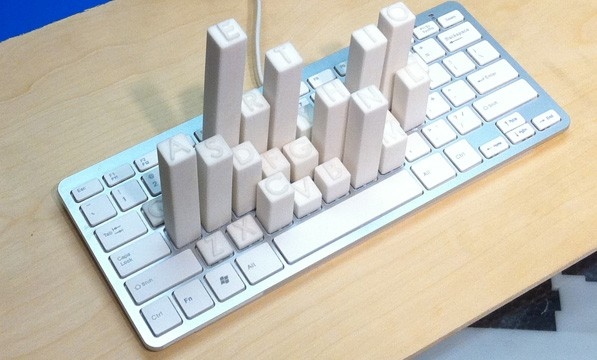
\includegraphics[width=0.6\textwidth]{keyboardfreq}
  \caption{Keyboard Frequency Sculpture}
  \label{fig:keyboardfreq}
\end{figure}

\subsection{Living Map: Precipitation Visualized with Moss}
Mappa ``vivente" che mostra il cambiamento nella quantità di precipitazioni nelle varie zone d'Europa a seguito del riscaldamento climatico
mediante l'erogazione controllata di acqua su un particolare tipo di muschio.  \cite{physlist}, Figura~\ref{fig:livingmap}.
\begin{figure}[h]
  \centering
  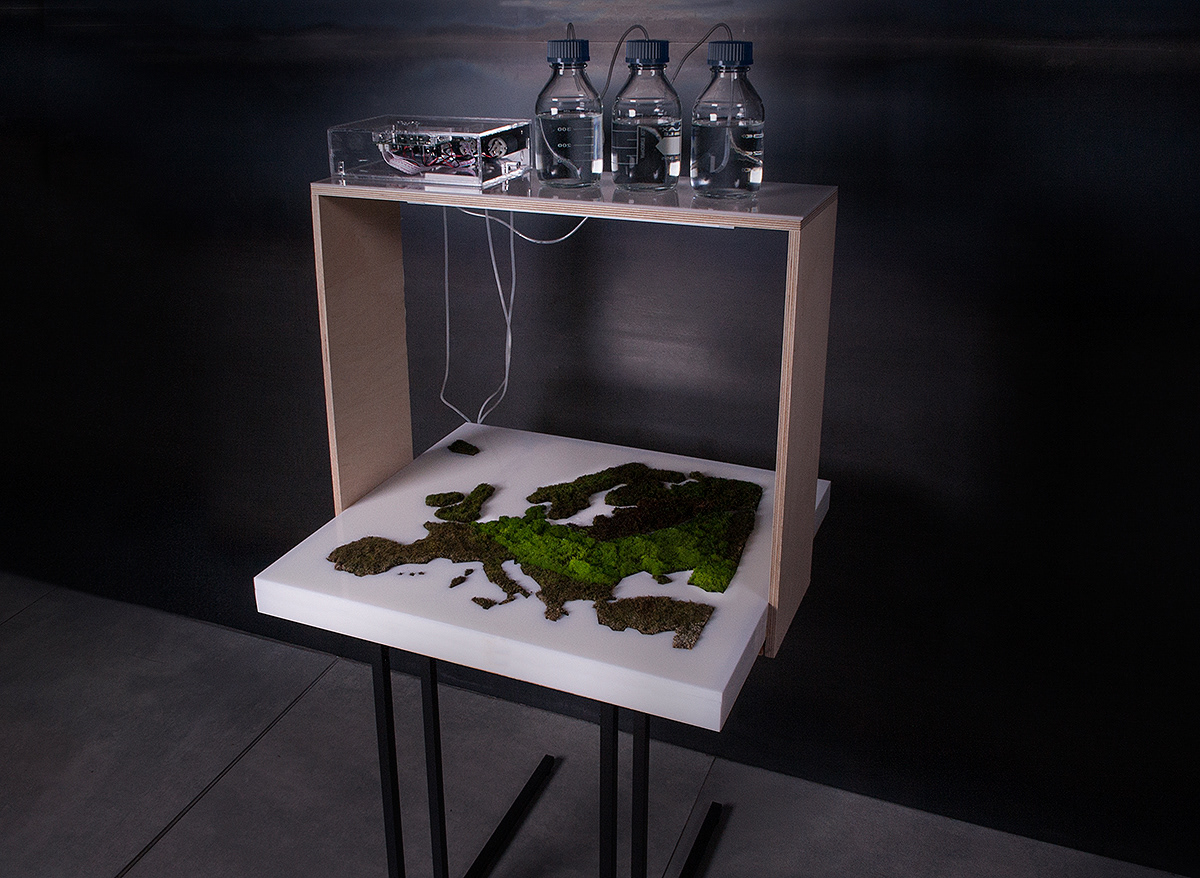
\includegraphics[width=0.8\textwidth]{livingmap}
  \caption{Living Map: Precipitation Visualized with Moss}
  \label{fig:livingmap}
\end{figure}

\subsection{Self Knitted Scarf of Train Delays}
Sciarpa lavorata a maglia da una pendolare di Monaco di Baviera con sezioni di colore diverso in base all'entità dei ritardi dei treni.
\cite{physlist}, Figura~\ref{fig:scarfdelays}.
La grossa sezione rossa è dovuta a un periodo di cantieri ferroviari in cui il treno era sostituito da un autobus.

\begin{figure}[h]
  \centering
  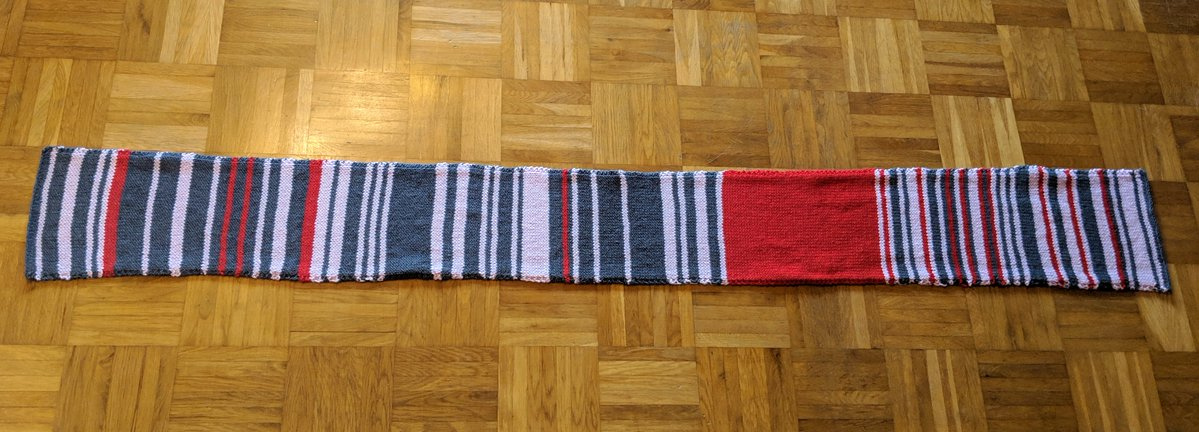
\includegraphics[width=0.8\textwidth]{scarfdelays}
  \caption{Self Knitted Scarf of Train Delays}
  \label{fig:scarfdelays}
\end{figure}

\subsection{Physiradio}
Una radio vintage che riproduce musica di mood/genere correlato alle condizioni metereologiche. \cite{physiradio}, Figura~\ref{fig:physiradio}.
\begin{figure}[h]
  \centering
  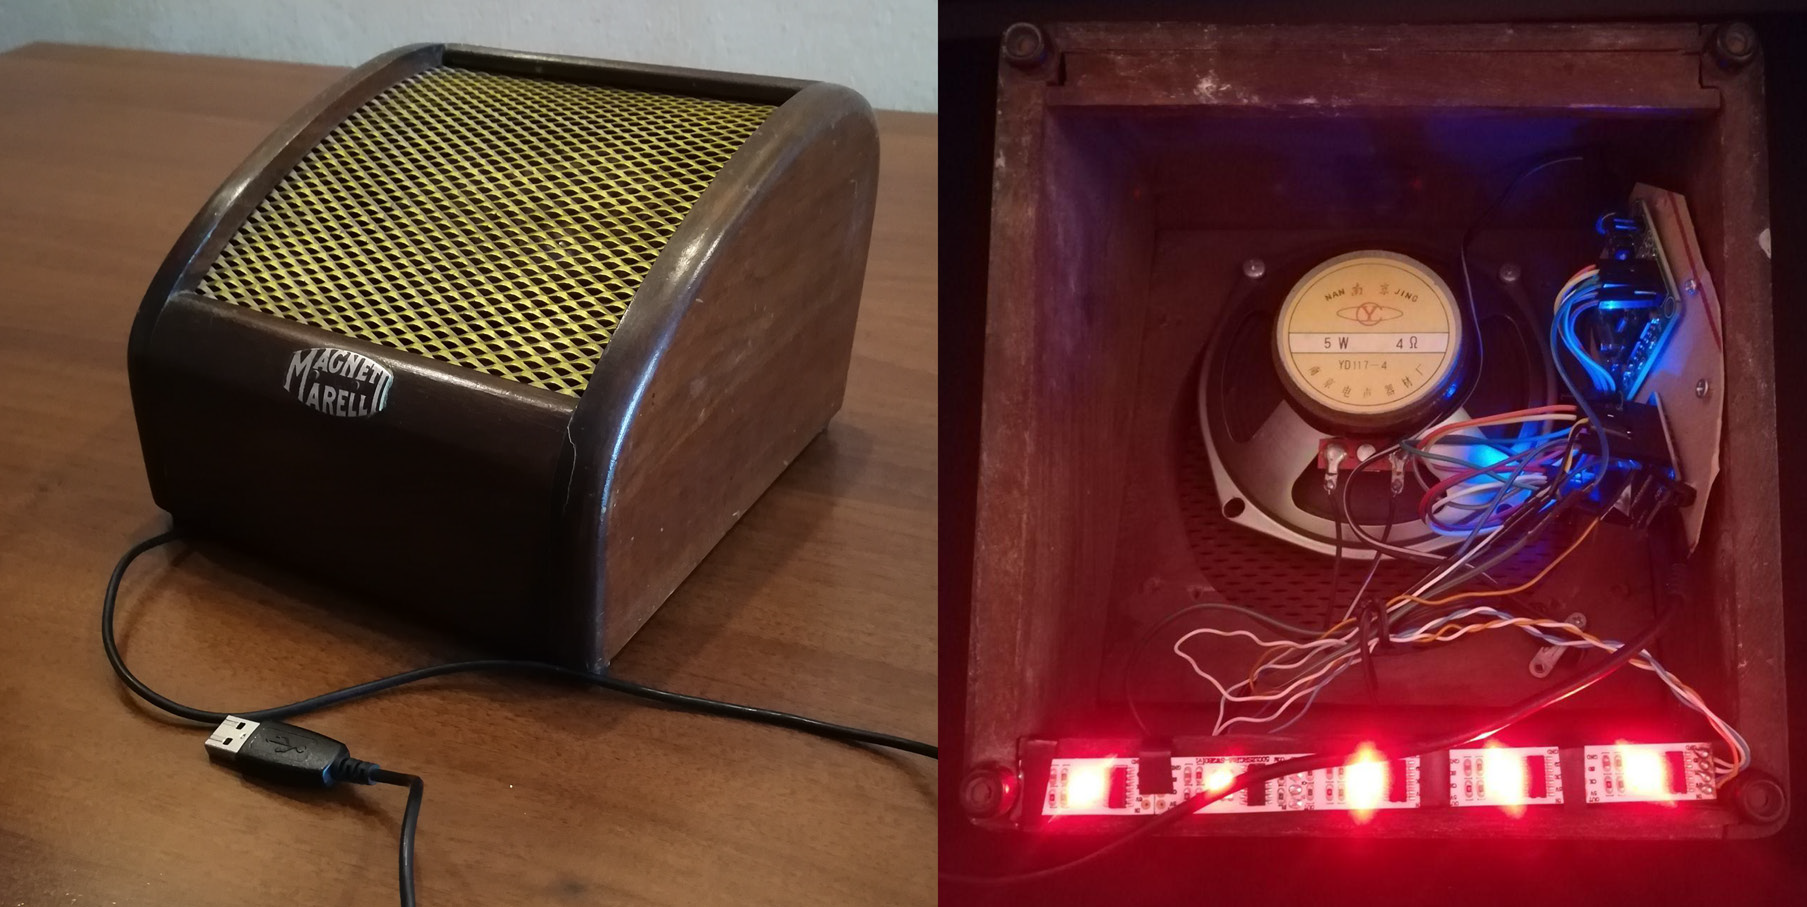
\includegraphics[width=0.8\textwidth]{physiradio}
  \caption{Physiradio}
  \label{fig:physiradio}
\end{figure}

\subsection{BiblioVisualizer}
Visualizzazione dei dati sul prestito libri nel consorzio Culture Socialità Biblioteche Network Operativo (CSBNO) tramite barra di LED.
\cite{bibliovisgitlab}, Figura~\ref{fig:bibliovisualizer}.
\begin{figure}[h]
  \centering
  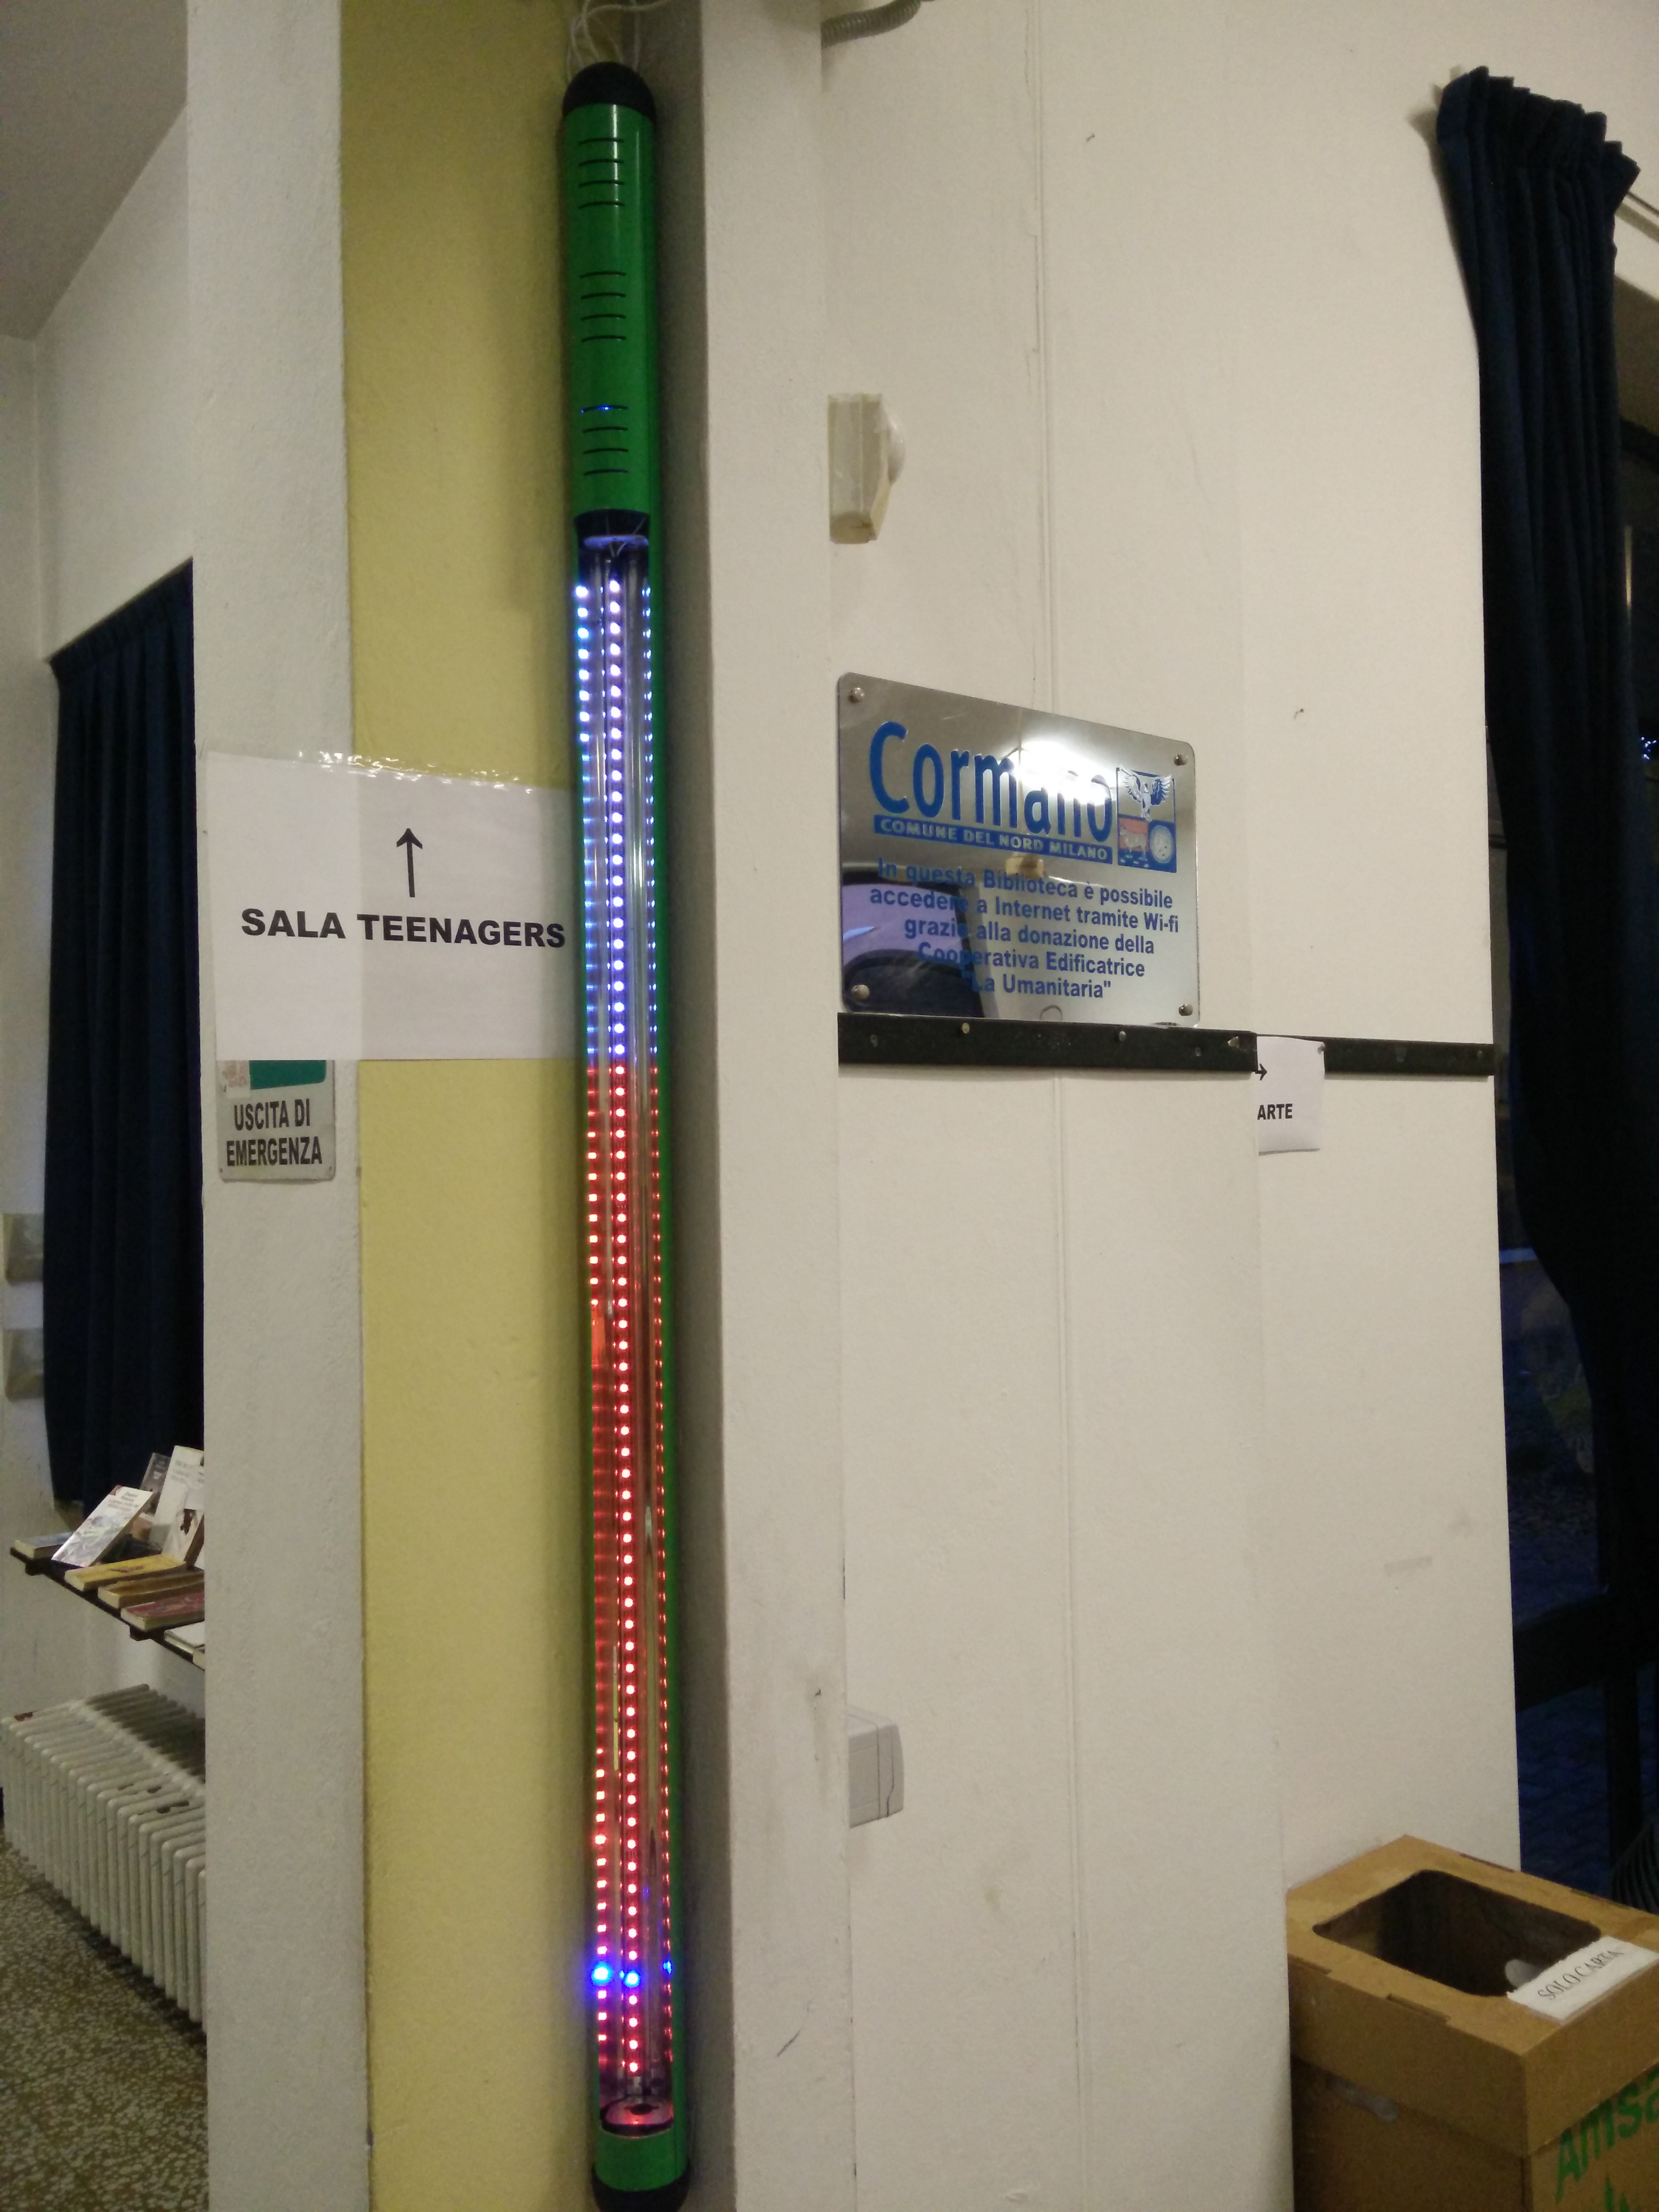
\includegraphics[width=0.5\textwidth]{bibliovisualizer}
  \caption{BiblioVisualizer}
  \label{fig:bibliovisualizer}
\end{figure}

\section{Internet of Things - IoT}
Concetto introdotto da Kevin Ashton nel 1999 e successivamente entrato nell'uso comune. Letteralmente: ``Internet delle cose",
si riferisce a una visione di Internet in cui non sono presenti solo persone a produrre e consumare informazioni ma
sono connessi anche oggetti (\emph{cose}), i quali sono molto più adeguati rispetto alle persone per catturare dati dal mondo reale
e scambiarseli.
\cite{ashton2009internet}

\section{ESP8266}
Microcontrollore economico e versatile, che comprende al suo interno funzionalità WiFi, un completo stack di rete, 17 pin General
Purpose (GPIO), supporta vari protocolli di comunicazione come I2C e possiede un ADC (Analog to Digital Converter) a 10 bit.
\cite{esp8266}.

Lo sviluppo hardware e software del prototipo che verrà illustrato nei seguenti capitoli è stato svolto su un Wemos D1 Mini, basato
su ESP8266.

\section{MQTT}
MQTT (Message Queuing Telemetry Transport) è un protocollo di messaggistica basato su publish/subscribe molto utilizzato in ambito
IoT per via della sua semplicità di implementazione, bassi requisiti prestazionali ed elevate scalabilità e affidabilità. 

L'architettura publish/subscribe si fonda sull'utilizzo di un broker centrale a cui i vari client si connettono e si scambiano messaggi
divisi per topic (argomenti) \cite{mqttorg}. Schema architetturale in Figura~\ref{fig:mqttarch}.

\begin{figure}[h]
  \centering
  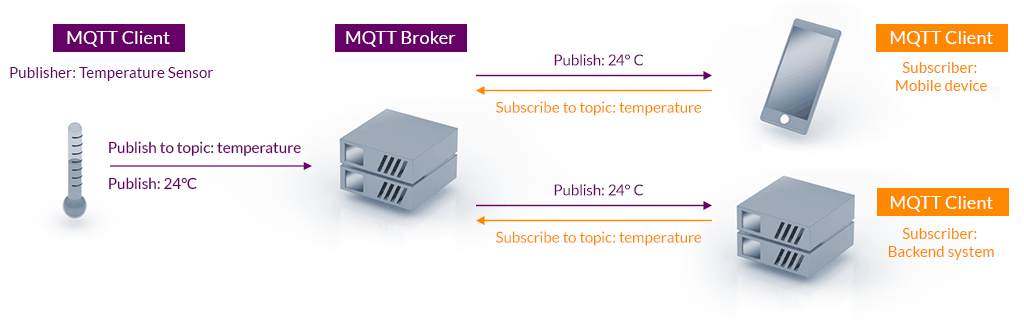
\includegraphics[width=\textwidth]{mqttarch}
  \caption{Architettura publish/subscribe di MQTT \cite{mqttorg}}
  \label{fig:mqttarch}
\end{figure}

\section{Obiettivo}
L'obiettivo dell'attività svolta durante il tirocinio è quello di analizzare e sperimentare una forma di fisicalizzazione
dei dati mediante strumenti di misura vintage e dispositivi IoT che non richieda l'utilizzo di computer e monitor e sia di semplice fruizione
da parte di chi non è avvezzo alla tecnologia e può essere intimorito da complicate dashboard (esempio in Figura~\ref{fig:datadash})
o semplicemente privo della volontà di interagire con dispositivi tecnologici per l'ottenimento di certe informazioni.
L'utilizzo di strumenti vintage consente infatti di ottenere oggetti discreti che possono far parte dell'arredamento domestico,
ad esempio su una mensola, i quali invece di essere puramente decorativi comunicano informazioni utili.

\begin{figure}[h]
  \centering
  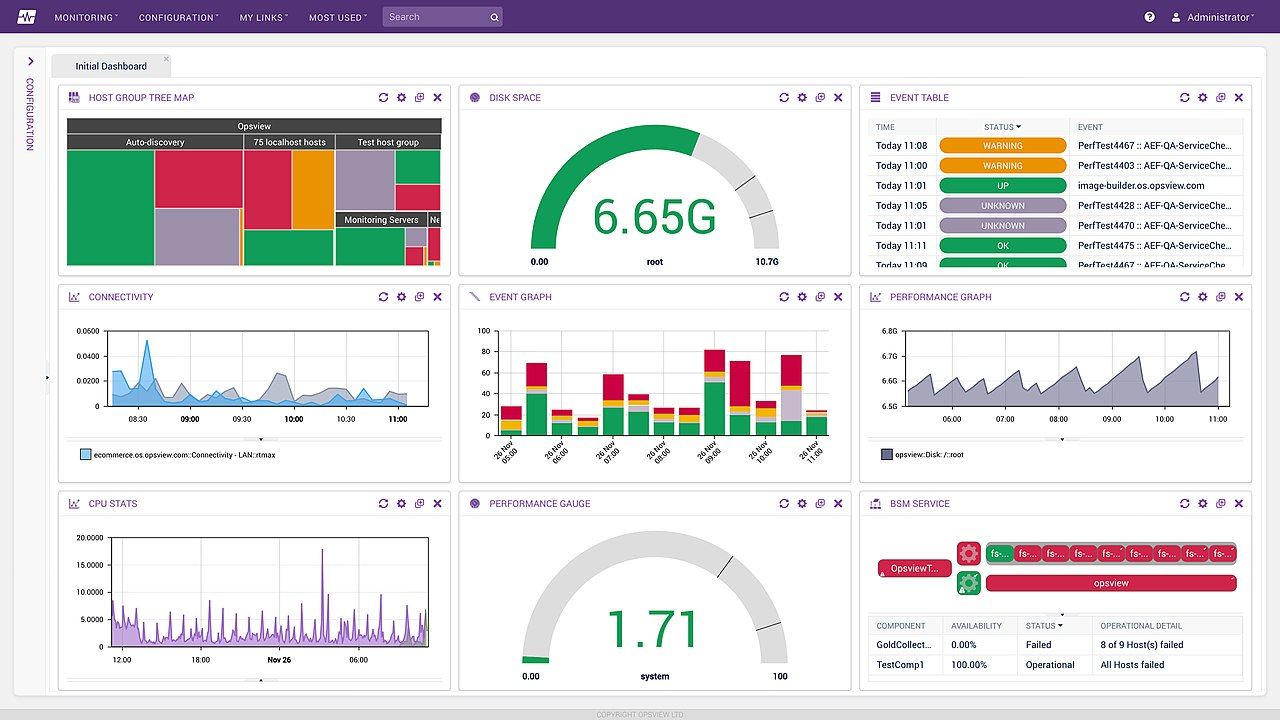
\includegraphics[width=\textwidth]{datadash}
  \caption{Esempio di dashboard data-oriented \cite{wiki:datadash}}
  \label{fig:datadash}
\end{figure}

\section{Esempi di riutilizzo di strumenti \textit{vintage}}% atrent cambiato titolo
La conversione di strumenti vintage per utilizzi diversi dall'originale è un'attività già svolta in passato da diverse persone. In questa
sezione verranno riportati alcuni esempi di esperimenti e prototipi e poi verranno descritte alcune delle piattaforme di sviluppo disponibili
per ESP8266.

%\todo{atrent: aggiungerne qualcuno (ispirazione hackaday, steampunk)}

\subsection{Retrofitting of an old tester from 1955}
Trasformazione di un vecchio tester in orologio, luce notturna e sveglia utilizzando un Arduino Nano con un ESP8266-01. 
\cite{retrofit1955}, Figura~\ref{fig:retrofit1955}.

\begin{figure}[h]
  \centering
  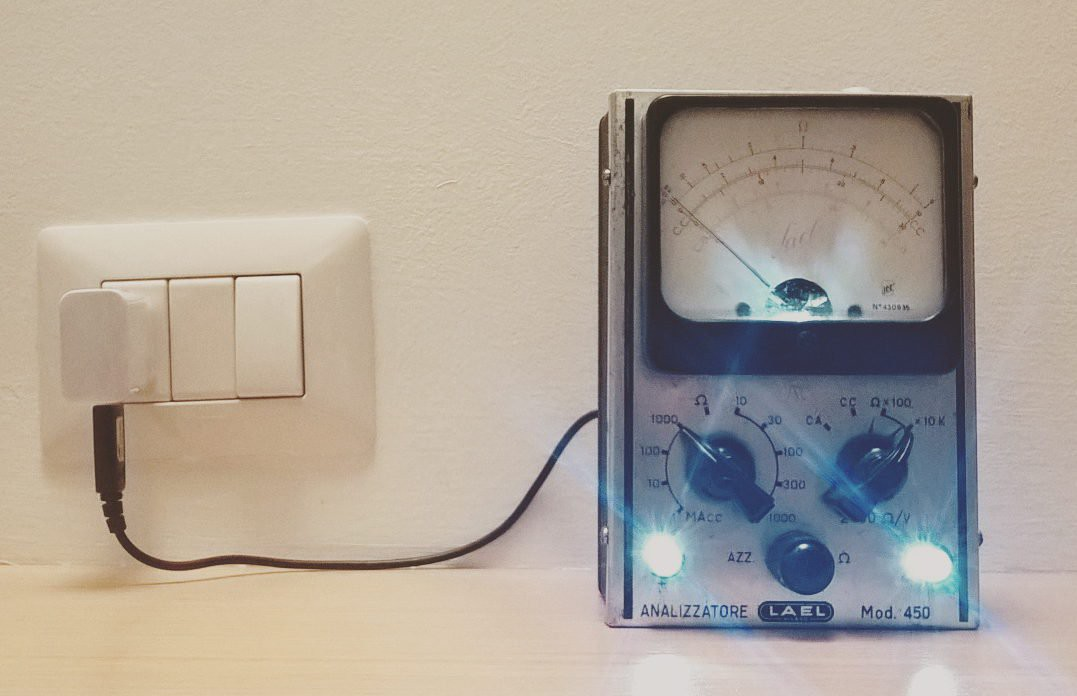
\includegraphics[width=0.7\textwidth]{retrofit1955}
  \caption{Retrofitting of an old tester from 1955 \cite{retrofit1955}}
  \label{fig:retrofit1955}
\end{figure}

\subsection{ESP8266 WiFi NTP voltmeter clock}
Orologio a 12 ore realizzato utilizzando tre voltmetri separati per ore, minuti e secondi. Le etichette sono state adattate per avere un intervallo
tra 1 e 12 per le ore e tra 0 e 60 per i minuti e secondi. L'ora viene ottenuta da Internet mediante una connessione WiFi e un server NTP.
\cite{voltclock}, Figura~\ref{fig:voltclock}.

\begin{figure}[h]
  \centering
  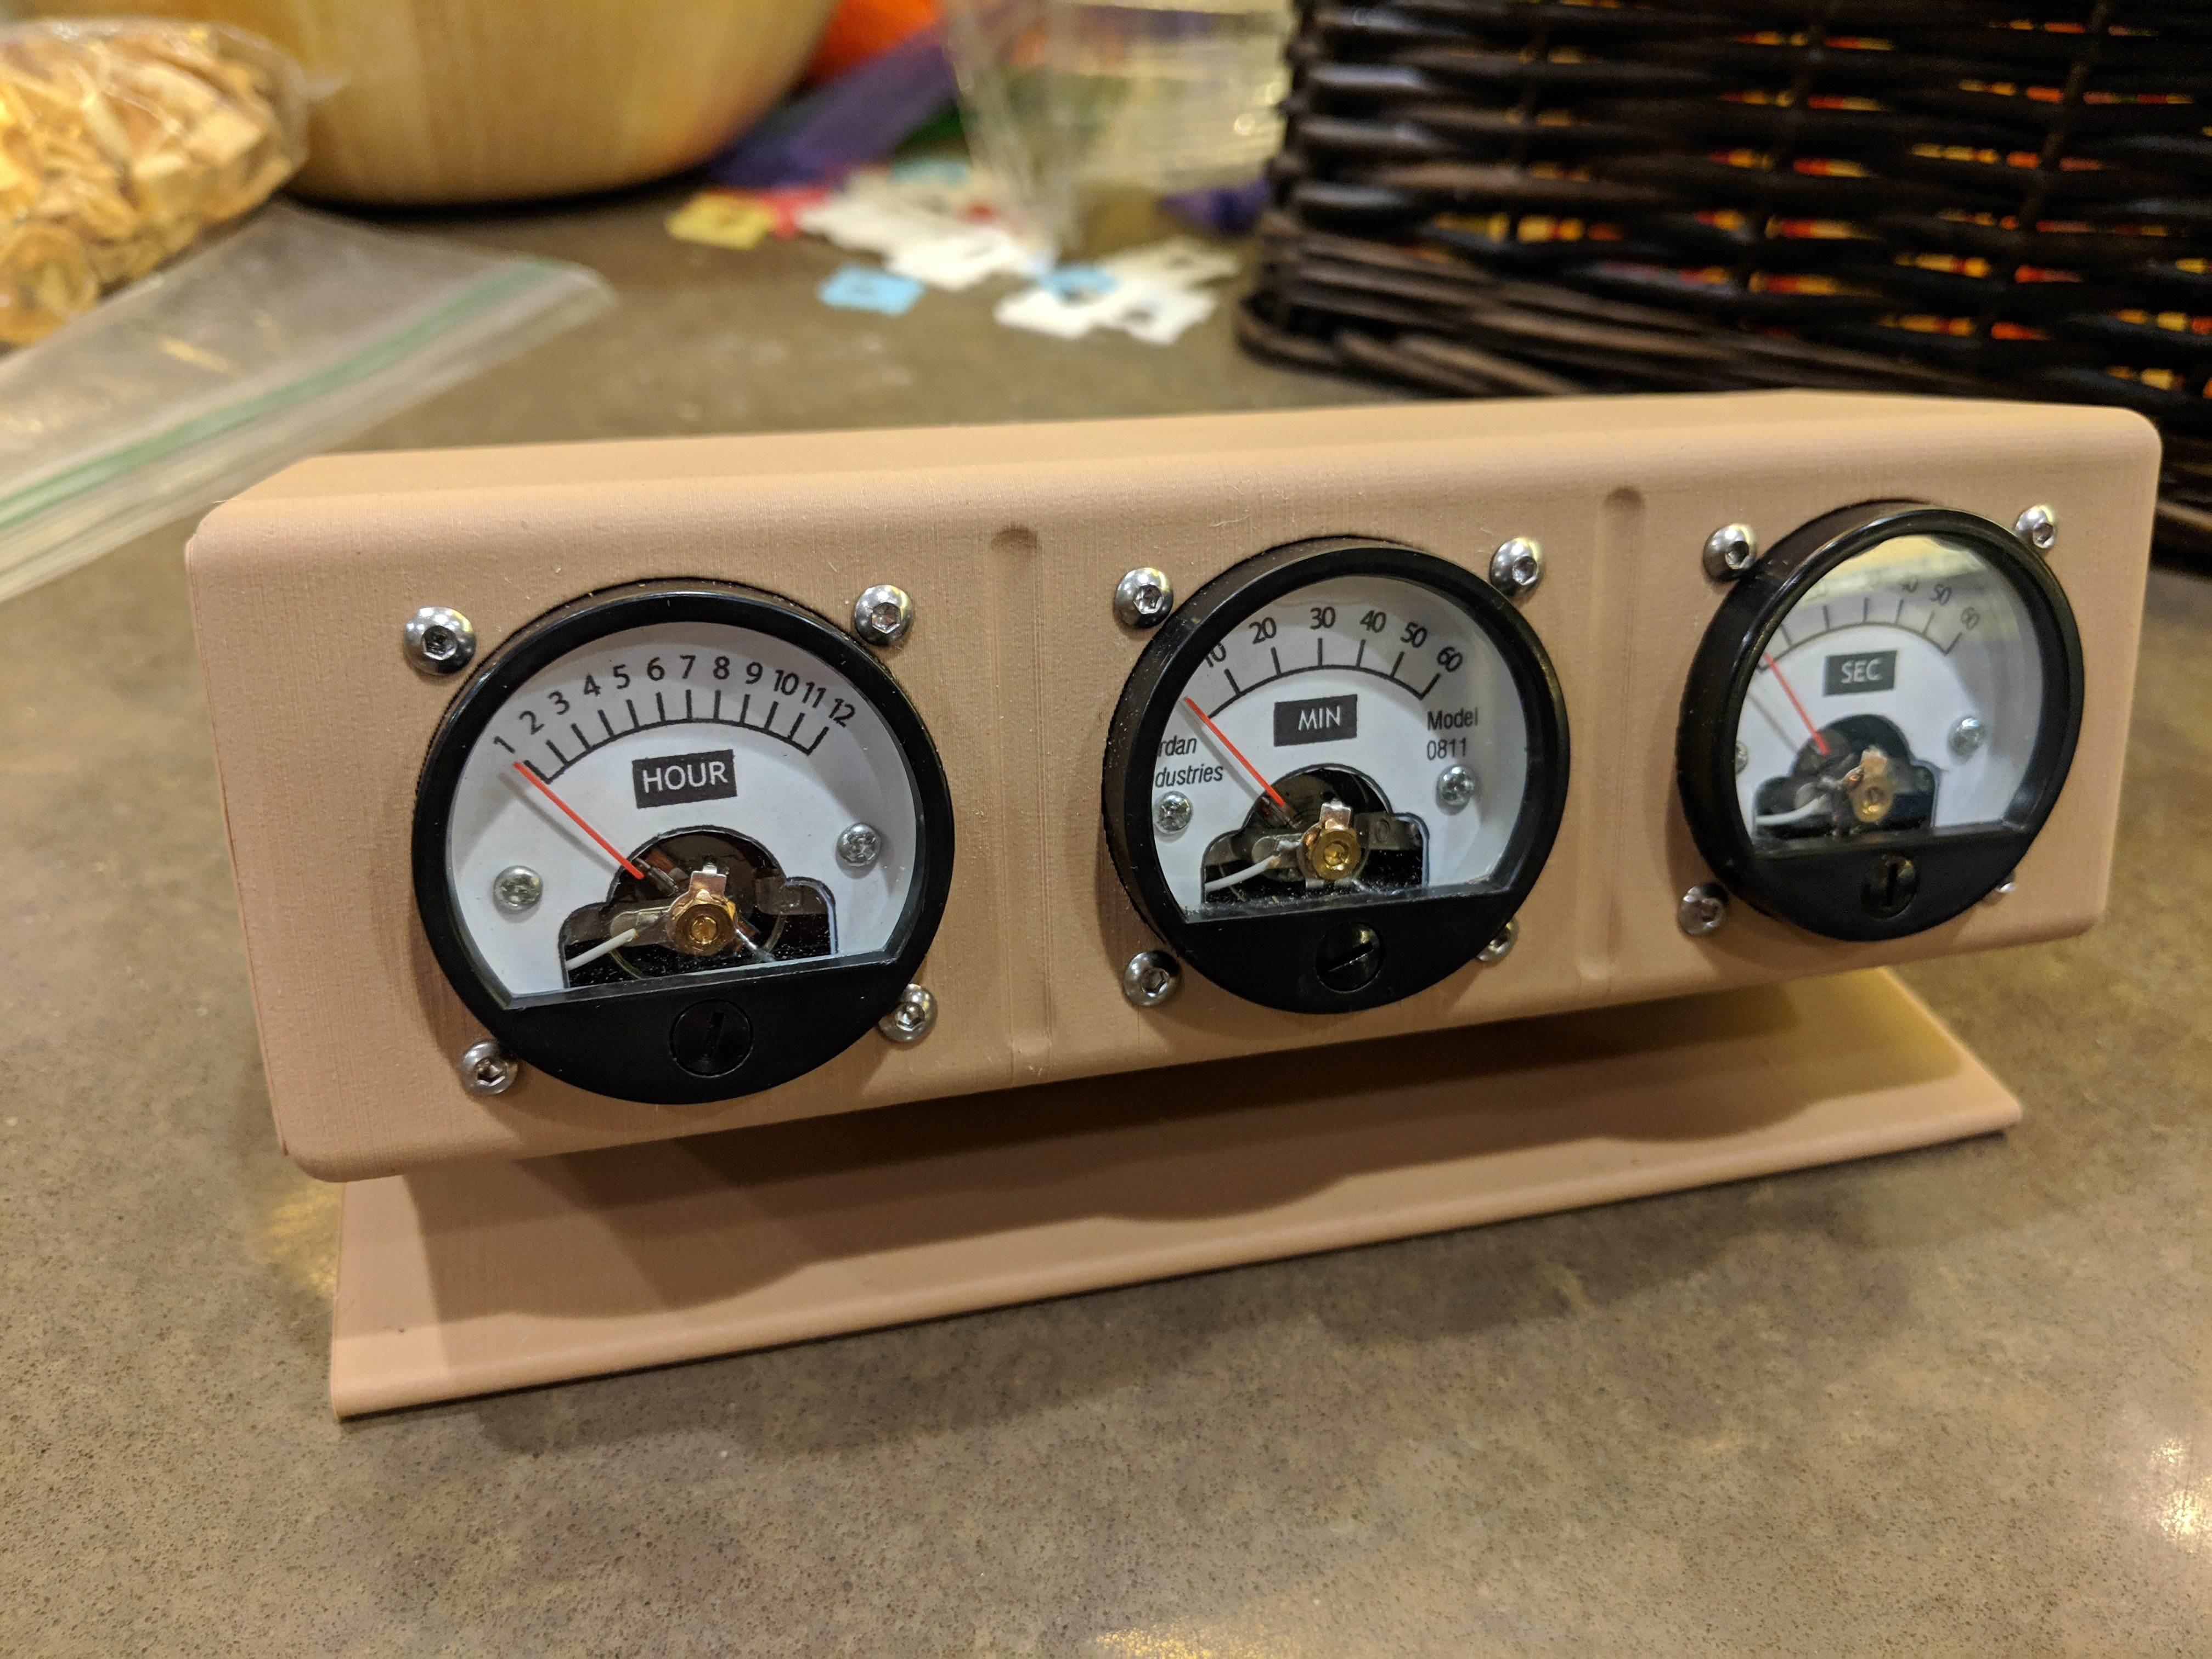
\includegraphics[width=0.7\textwidth]{voltclock}
  \caption{ESP8266 WiFi NTP voltmeter clock  \cite{voltclock}}
  \label{fig:voltclock}
\end{figure}


\subsection{MQTT controlled analog gauge ``vintage style"}
Basato su ESP8266 e mongoose-os. Controllato mediante MQTT, produce un'uscita PWM che viene visualizzata tramite l'ago del voltmetro,
appositamente modificato per avere una taratura sul voltaggio del microcontrollore invece che su 110V.
Questa modifica è molto simile a quelle che verranno affrontate nelle prossime sezioni.
\cite{gaugevintagestyle}, Figura~\ref{fig:gaugevintagestyle}.

\begin{figure}[h]
  \centering
  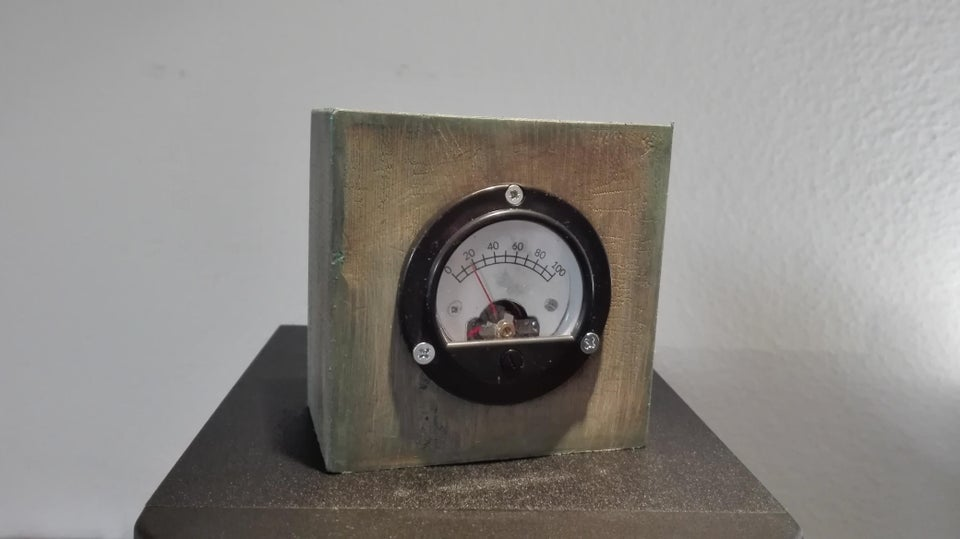
\includegraphics[width=0.8\textwidth]{gaugevintagestyle}
  \caption{MQTT controlled analog gauge ``vintage style" \cite{gaugevintagestyle}}
  \label{fig:gaugevintagestyle}
\end{figure}

\subsection{Ampere time}
Orologio giornaliero realizzato utilizzando un vecchio amperometro per la didattica. Il fatto che le intere 24 ore siano ``schiacciate"
in un intervallo ristretto, secondo l'autore, è un buon antidoto agli stressanti ritmi della vita moderna.
\cite{amperetime}, Figura~\ref{fig:amperetime}.

\begin{figure}[h]
  \centering
  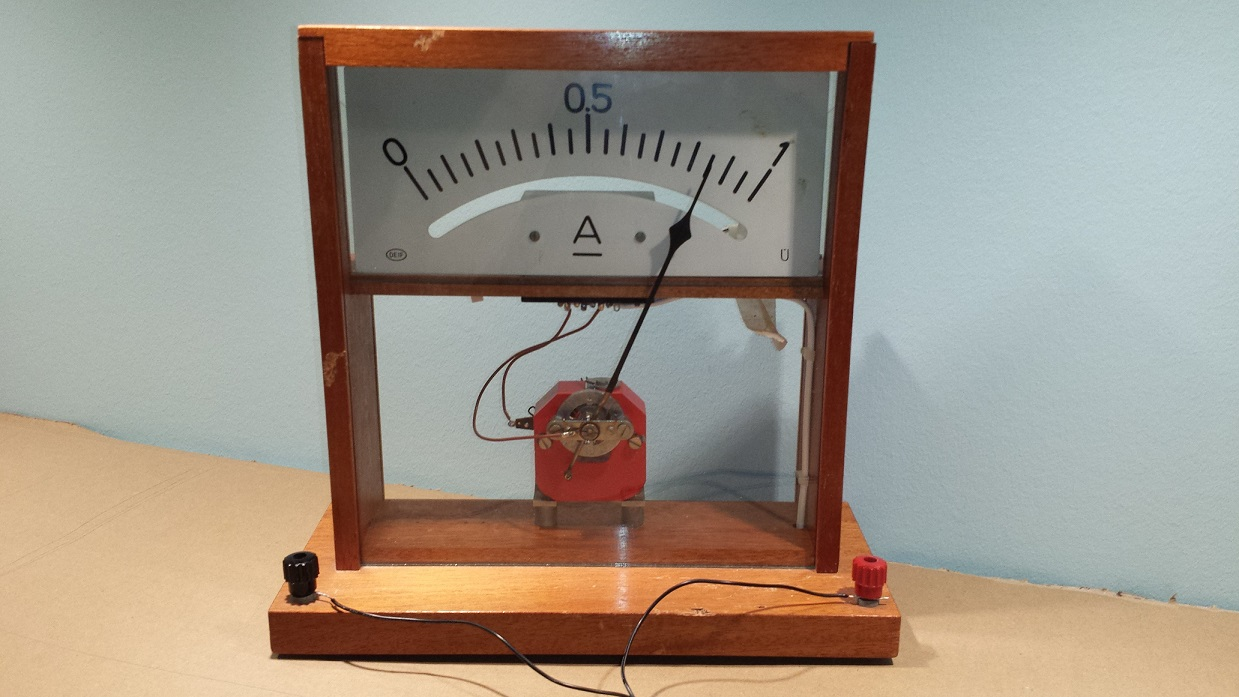
\includegraphics[width=0.8\textwidth]{amperetime}
  \caption{Ampere time \cite{amperetime}}
  \label{fig:amperetime}
\end{figure}

\subsection{Retro Nixie Tube Clock}
Un orologio rétro in stile Steampunk basato su valvole Nixie, tubi in rame e legno riciclato.
\cite{nixieclock}, Figura~\ref{fig:nixieclock}.

\begin{figure}[h]
  \centering
  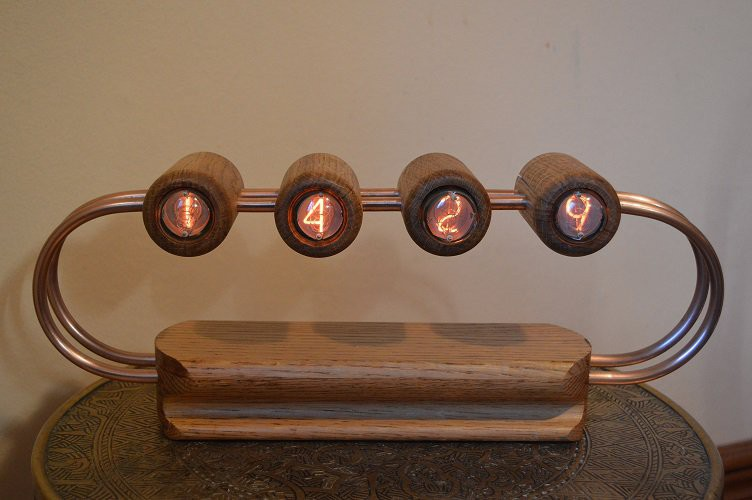
\includegraphics[width=0.8\textwidth]{nixieclock}
  \caption{Retro Nixie Tube Clock \cite{nixieclock}}
  \label{fig:nixieclock}
\end{figure}

\subsection{aPCmeter}
Progetto in stile vintage che consiste in indicatori basati su voltmetri DC pilotati tramite un Arduino Nano usati per riportare lo stato di
utilizzo di CPU e RAM del PC. I voltmetri sono illuminati da LED RGB il cui colore cambia in base al valore rappresentato.
\cite{apcmeter}, Figura~\ref{fig:apcmeter}.

\begin{figure}[h]
  \centering
  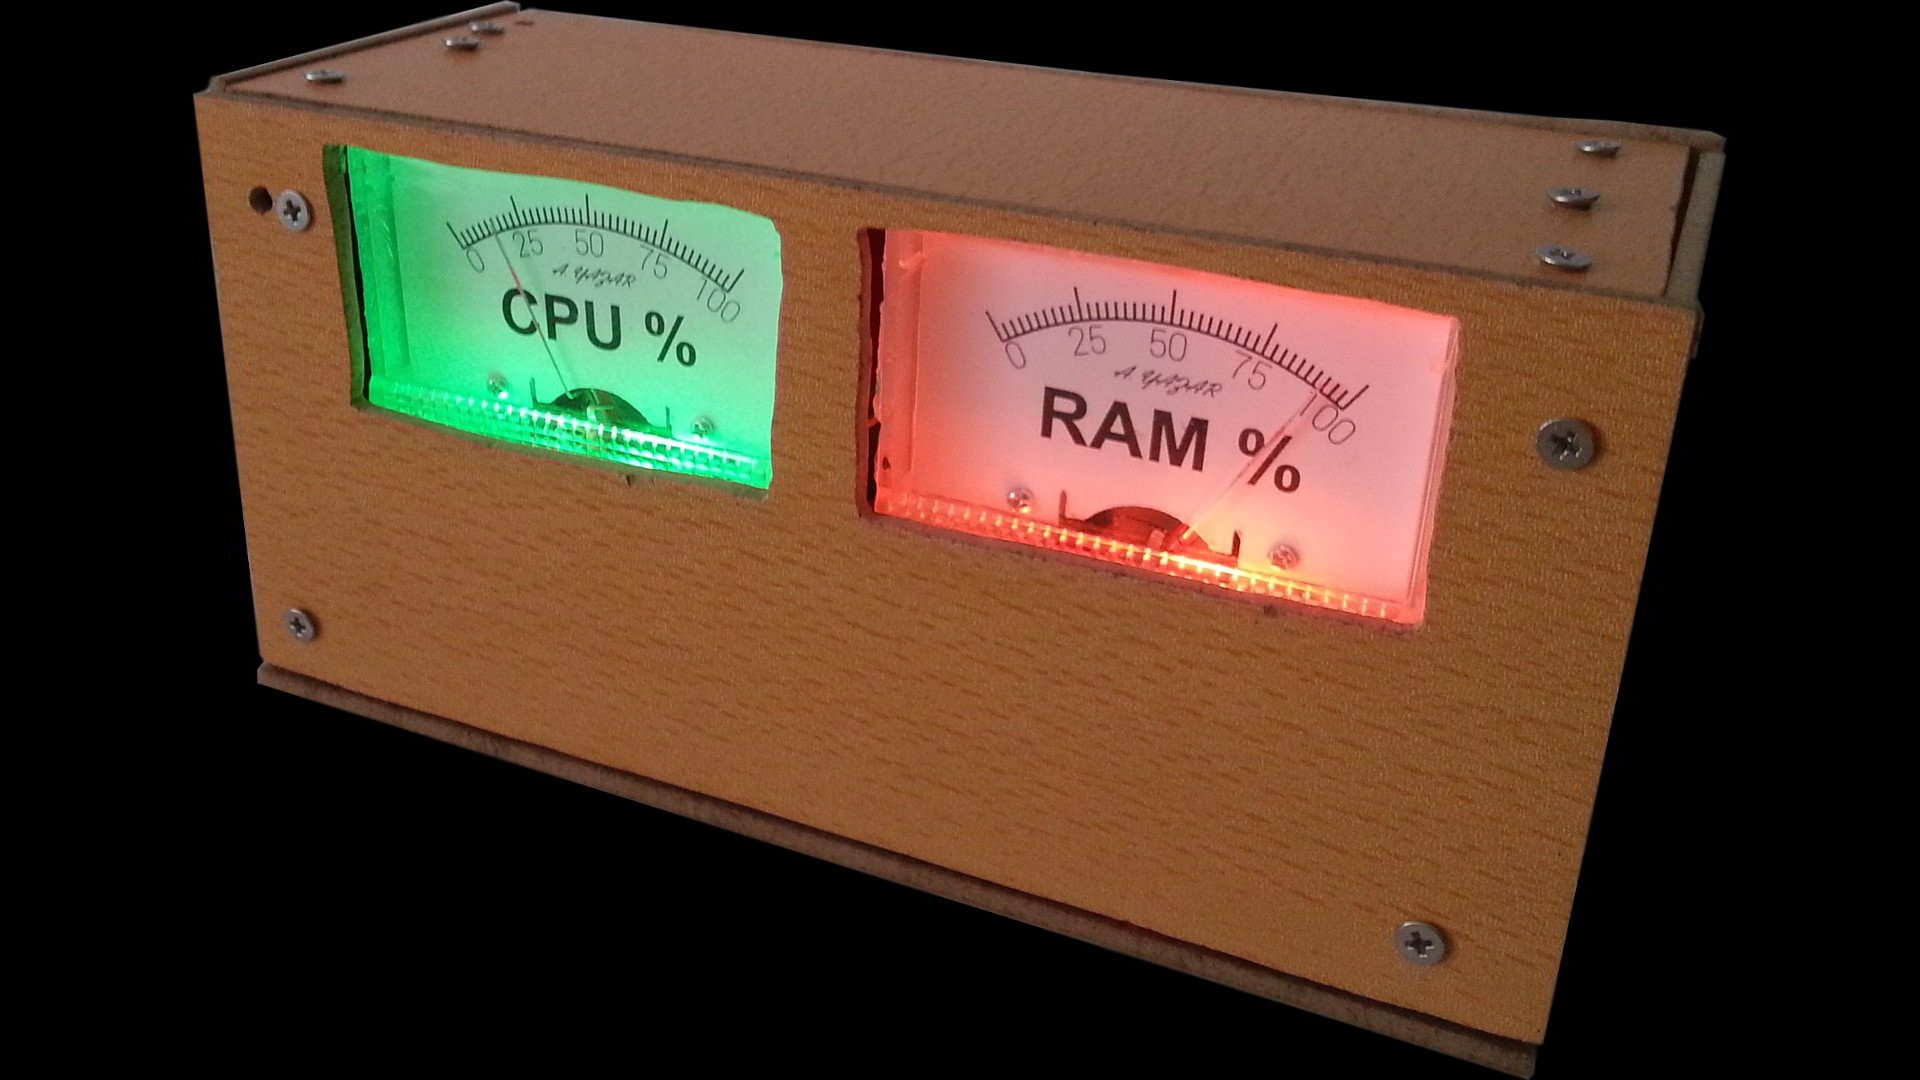
\includegraphics[width=0.8\textwidth]{apcmeter}
  \caption{aPCmeter \cite{apcmeter}}
  \label{fig:apcmeter}
\end{figure}


%\todo{atrent: questa sotto e le seguenti forse dovevano essere delle section?}
\section{Tasmota}
Tasmota è un firmware open source per dispositivi basati su ESP8266, nato come espansione per il firmware degli interruttori
wireless Sonoff al fine di arricchirli con funzionalità MQTT. Il suo obiettivo è quello di rendere più configurabili e controllabili i dispositivi
smart, mediante interfaccia web, MQTT, KNX e integrazioni con i vari sistemi di home automation.
\cite{abouttasmota}.

\section{ESPHome}
ESPHome è un sistema per creare firmware personalizzato per dispositivi ESP8266 e ESP32 tramite semplici file di configurazione e poi controllarli
da remoto mediante sistemi di Home Automation.
Supporta una grande quantità di componenti hardware e software il che lo rende particolarmente versatile per una vastissima gamma di utilizzi
\cite{esphomeio}.
Per alcune delle feature del prototipo realizzato durante il tirocinio è stato deciso di utilizzare questo sistema.

\section{Steampunk}
Vista l'attinenza con l'obiettivo del tirocinio, è il caso di menzionare anche la corrente artistica Steampunk, la quale si basa su
un'anacronistica idea di ``futuro" evoluto dall'epoca vittoriana in cui la tecnologia dominante è ancora il vapore (\emph{steam})
e i materiali di cui sono composti gli oggetti di uso comune rimangono l'ottone e il cuoio. \cite{focussteampunk}
Nelle opere di questo genere è molto comune trovare grandi tubi per il vapore e indicatori vari sparsi per ogni tipo di oggetto.
Esempio di oggetto Steampunk in Figura~\ref{fig:steampunklamp}
\todo{atrent: minimale, avrei detto qualcosa di più...}

\begin{figure}[h]
  \centering
  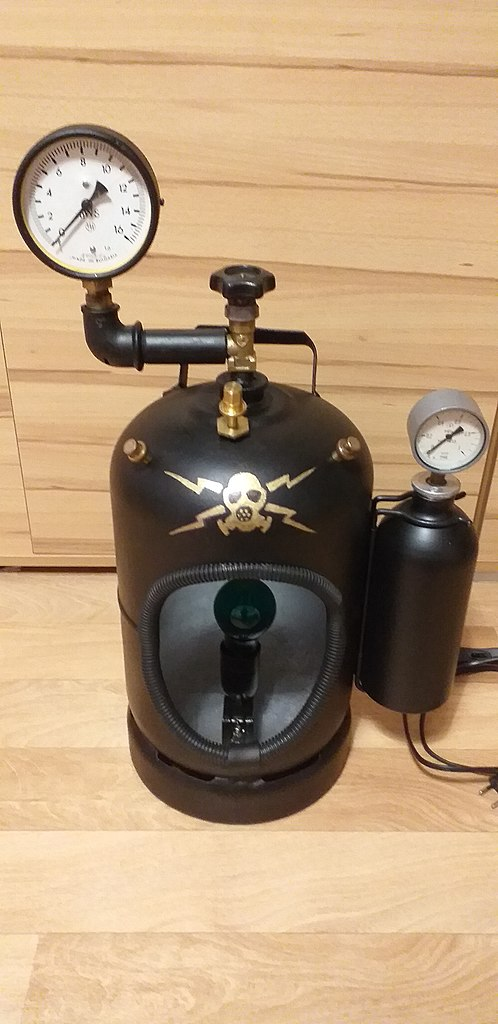
\includegraphics[width=0.7\textwidth]{steampunklamp}
  \caption{Bombola di gas convertita in lampada Steampunk \cite{wiki:steampunklamp}}
  \label{fig:steampunklamp}
\end{figure}

\chapter{Panoramica storica e caratteristiche fisiche degli strumenti}
%\todo{Sezione panoramica storica più caratteristiche fisiche, "istanze"}

\section{Strumenti}
\subsection{Strumenti ad ago}
Sono il tipo più comune di strumento di misura vintage. Un esempio sono i voltmetri / amperometri / multimetri analogici che si utilizzavano
fino a pochi anni fa. Possono essere utilizzati per visualizzare grandezze lineari, facendo attenzione alla scala scelta.
Panoramica in Figura~\ref{fig:strumentiago}.
\begin{figure}[h]
  \centering
  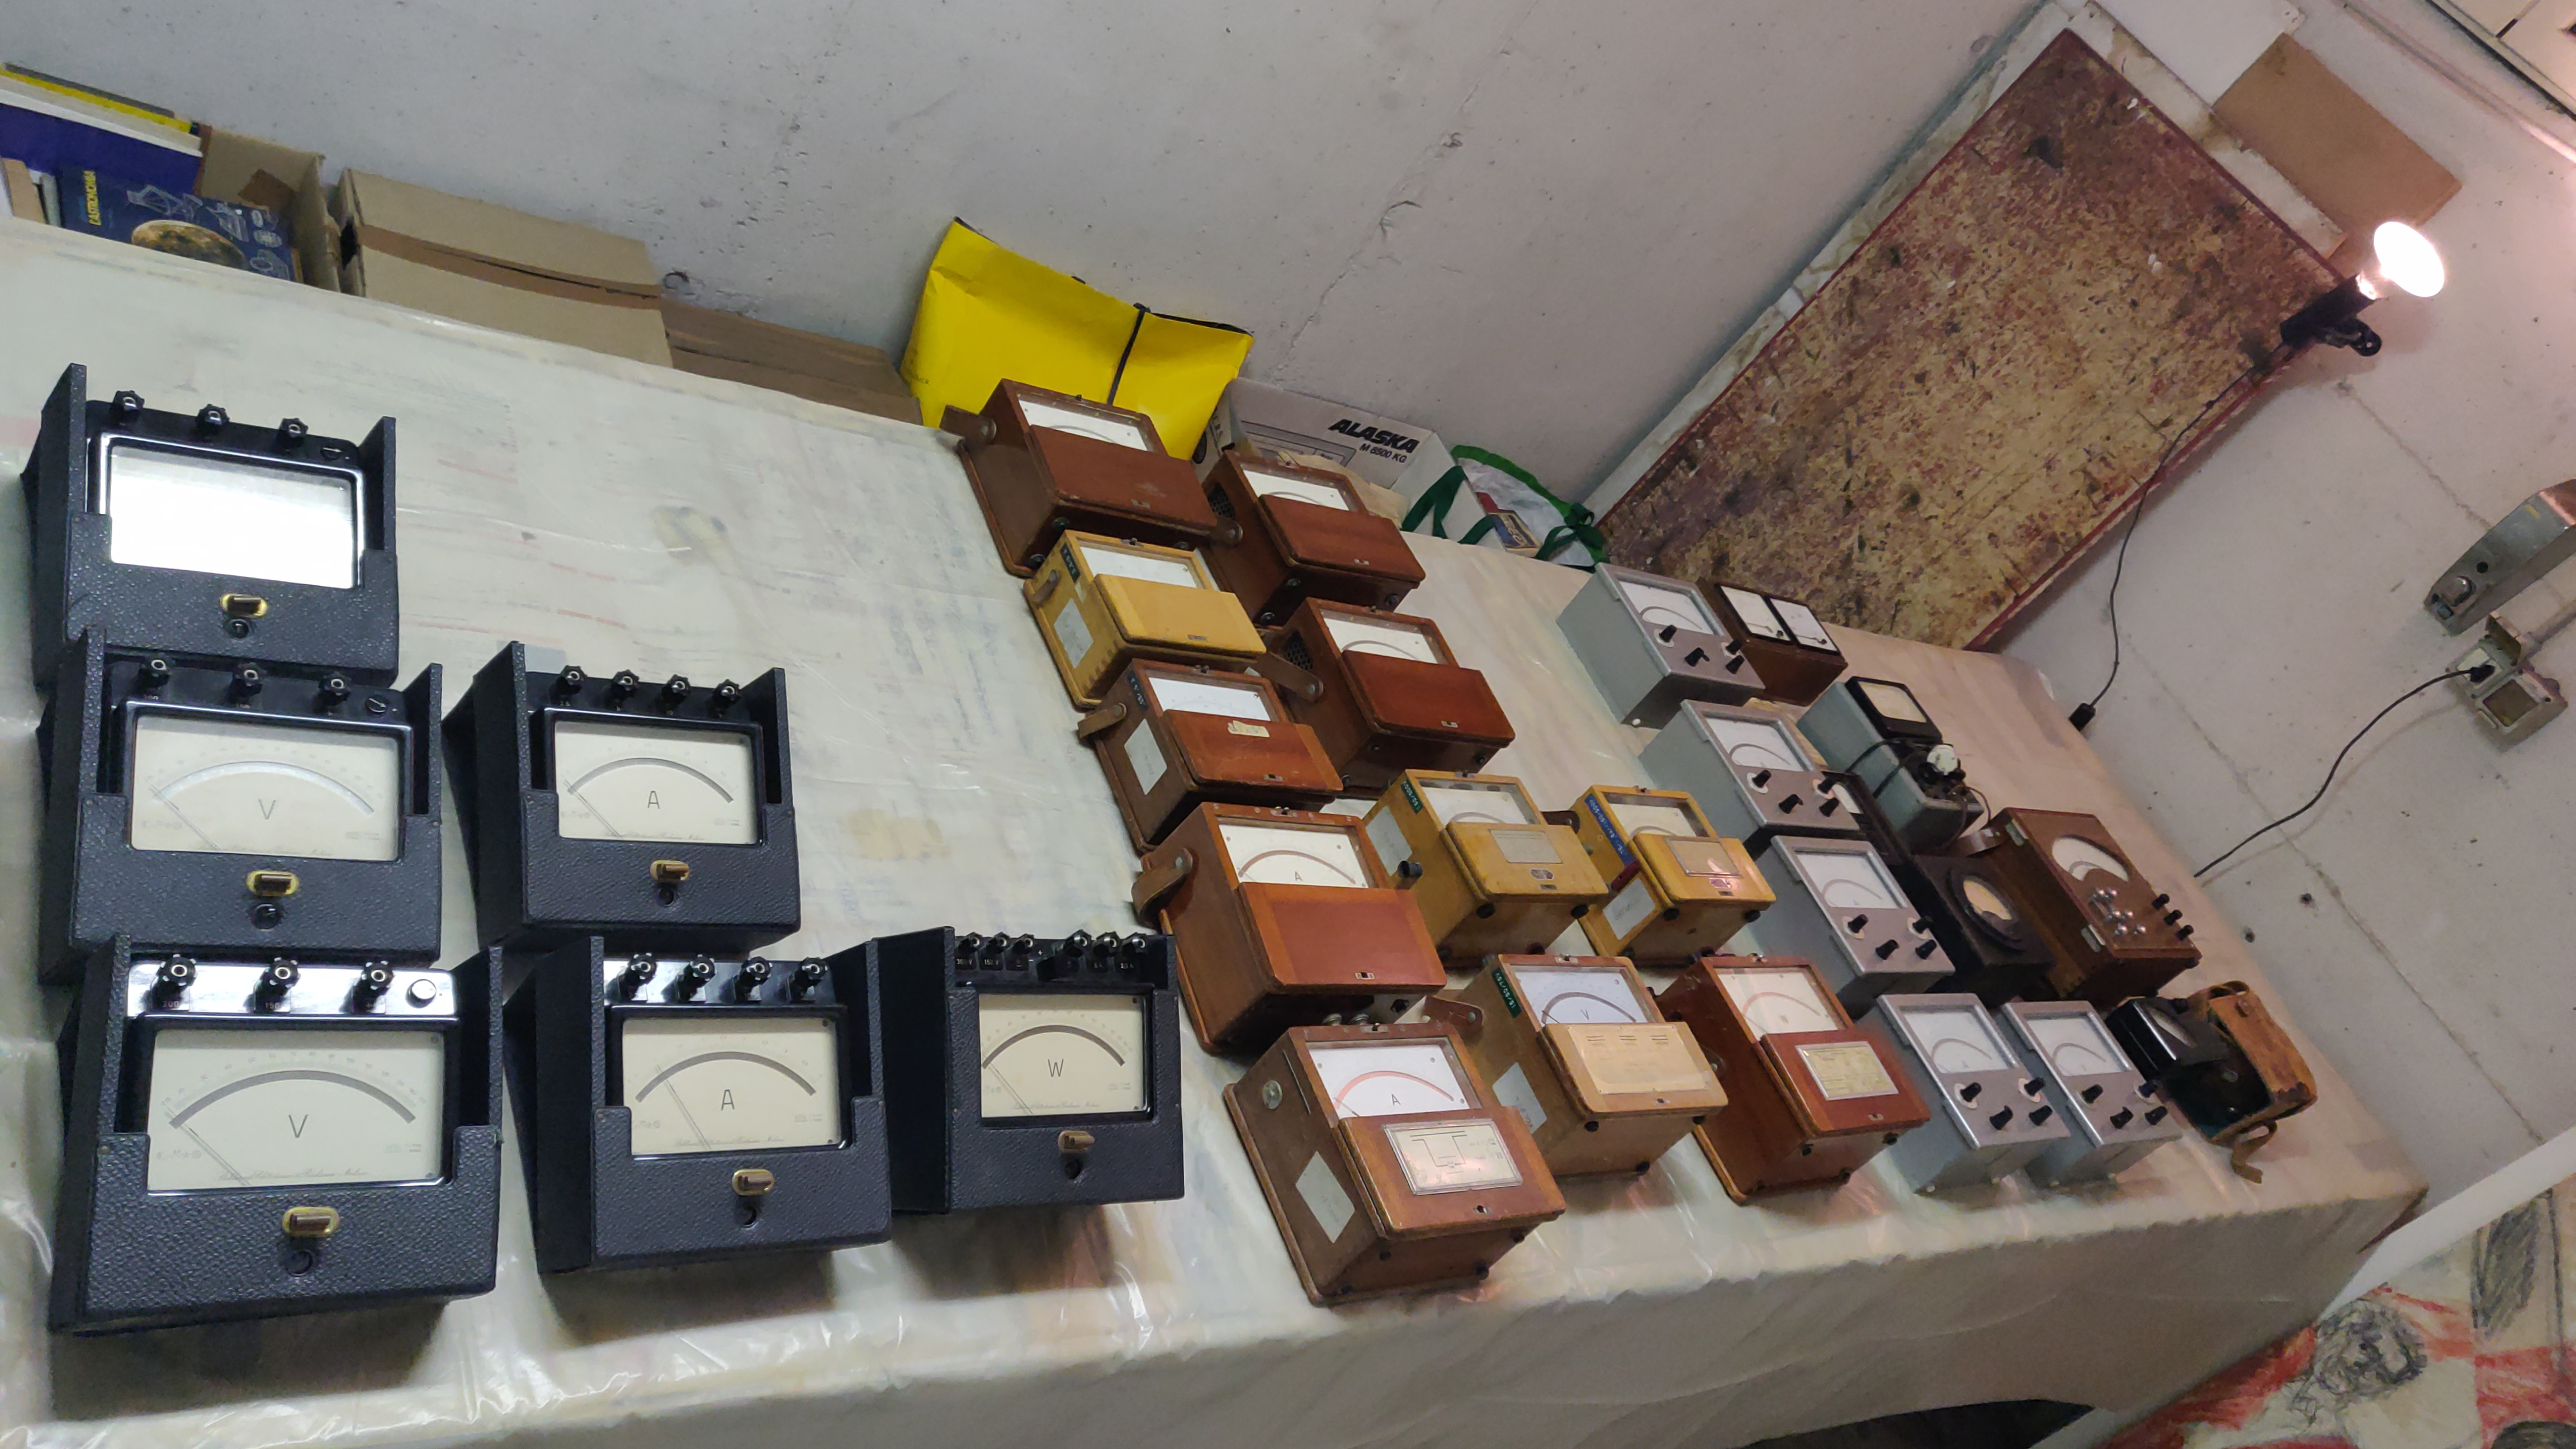
\includegraphics[width=0.9\textwidth]{strumentiago}
  \caption{Assortimento di strumenti ad ago in bachelite, legno e metallo}
  \label{fig:strumentiago}
\end{figure}

\paragraph{Funzionamento}
%generica per ora
Quasi tutti gli strumenti ad ago sono basati su milliamperometri, aventi una resistenza interna, integrati con resistenze di taratura
in serie e/o in parallelo in base all'utilizzo finale desiderato. Per ottenere un voltmetro con fondoscala adeguato, è spesso necessario
inserire una resistenza in serie con il milliamperometro, in modo da ridurne la sensibilità.
Questo principio si basa sulla legge di Ohm: conoscendo il flusso di corrente necessario normalmente per arrivare a fondo scala, è
possibile calcolare la resistenza totale necessaria per portare l'ago al 100\% in corrispondenza di una tensione desiderata.
Esempio di scheda resistenze in Figura~\ref{fig:schedaresistenze}.

\begin{figure}[h]
  \centering
  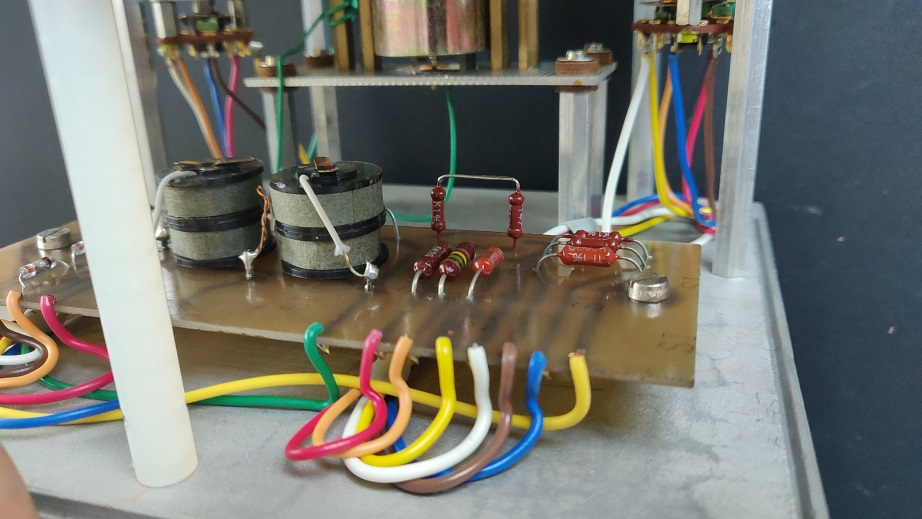
\includegraphics[width=0.8\textwidth]{schedaresistenze}
  \caption{Scheda resistenze di un voltmetro analogico}
  \label{fig:schedaresistenze}
\end{figure}


\subsection{Dekatron}
Valvola termoionica che svolge la funzione di dispositivo di conteggio, molto usata all'interno dei computer negli anni '50 e '60 e ora
relegata all'utilizzo hobbistico, ad esempio per la realizzazione di particolari orologi. \cite{itwiki:118300354}, Figura~\ref{fig:dekatron}.

\begin{figure}[h]
  \centering
  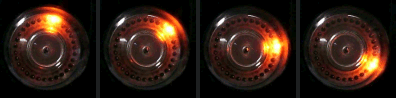
\includegraphics[width=0.9\textwidth]{dekatron}
  \caption{Dekatron \cite{itwiki:118300354}}
  \label{fig:dekatron}
\end{figure}

\subsection{Occhio magico}
Valvola termoionica usata per rappresentare l'intensità di un segnale elettrico. Storicamente impiegata nelle radio come
indicatore di sintonia. \cite{itwiki:119250611}, Figura~\ref{fig:occhiomagicofasi}.

\begin{figure}[h]
  \centering
  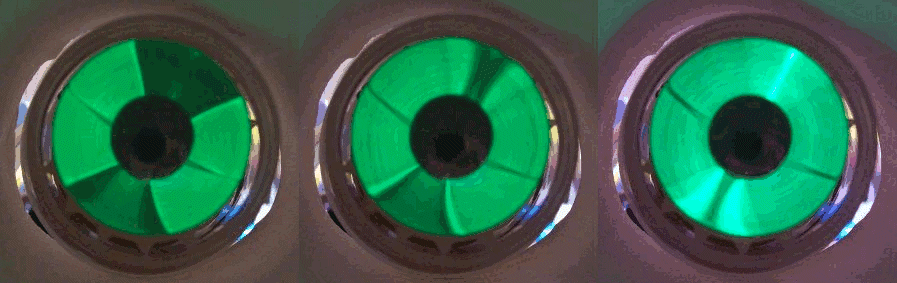
\includegraphics[width=0.9\textwidth]{occhiomagicofasi}
  \caption{Occhio magico in diverse fasi di illuminazione \cite{itwiki:119250611}}
  \label{fig:occhiomagicofasi}
\end{figure}

\subsection{Oscilloscopio}
Strumento utilizzato per visualizzare l'andamento nel tempo di un segnale in maniera grafica \cite{itwiki:120862120}. Se pilotato a dovere è in grado di
visualizzare delle grafiche. Esempio in Figura~\ref{fig:oscilloscopio}.

\begin{figure}[h]
  \centering
  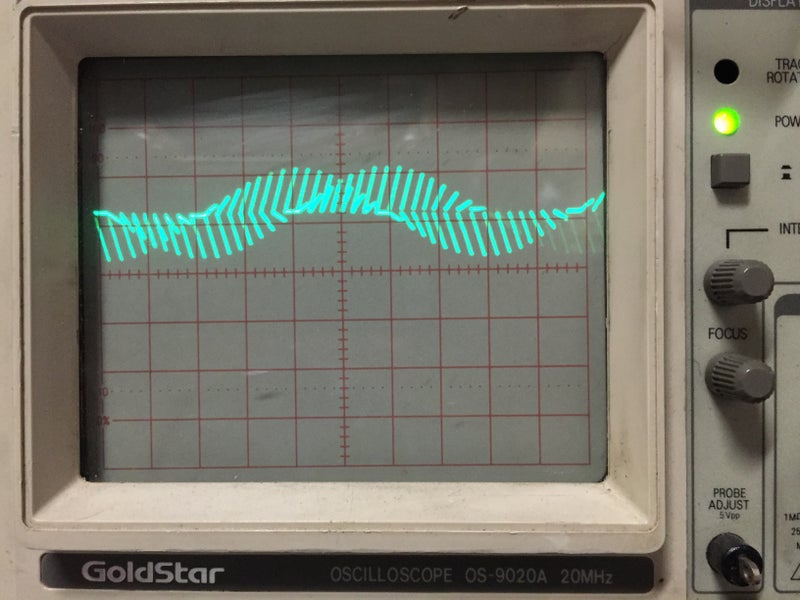
\includegraphics[width=0.8\textwidth]{oscilloscopio}
  \caption{Oscilloscopio impiegato nella visualizzazione di un disegno \cite{instructablesoscilloscope}}
  \label{fig:oscilloscopio}
\end{figure}

\section{Componenti}
In questa sezione si farà una panoramica dei componenti che si possono incontrare a bordo degli strumenti vintage. Alcuni hanno
un'utilità ai fini della fisicalizzazione o in generale alla conversione per l'utilizzo con microcontrollori, mentre altri non sono convertibili.

\todo{atrent: mettere un po' di foto dei vari componenti!}

%\todo{atrent: dire cosa intendi raccontare in questa sezione e dire che alcuni di questi NON saranno usabili}

\subsection{Interruttori / Pulsanti}
Formati da un semplice meccanismo che permette di aprire o chiudere un circuito.
\subsection{Commutatori a n posizioni}
Sono utilizzati per chiudere uno tra n possibili circuiti attraverso la loro rotazione e il conseguente spostamento di contatti elettrici.
Esempio in Figura~\ref{fig:commutatoreprimadopo}.
\subsection{Potenziometri}
Consentono di variare una differenza di potenziale nel continuo mediante un partitore resistivo ``mobile".
\subsection{Morsetti/Connettori}
Consentono di collegare e scollegare cavi o sonde allo strumento.
\subsection{Lampadine}
Fonte luminosa. Generalmente quelle che si possono trovare nei vecchi apparati sono piccole e a incandescenza. Contengono un filamento
metallico, spesso di tungsteno, che scaldandosi emette della luce.
\subsection{Altoparlanti}
Consentono di produrre suoni di varia natura, solitamente composti da una membrana che viene mossa da una bobina per generare onde
sonore. Richiedono amplificazione.
\subsection{Buzzer}
Dispositivi di segnalazione acustica, i più comuni sono di tipo piezoelettrico e producono un fischio generato da un circuito elettrico oscillante.
Sono spesso impiegati negli strumenti di misura ad esempio per segnalare continuità elettrica.
Interno di un buzzer in Figura~\ref{fig:internobuzzer}.

\begin{figure}[h]
  \centering
  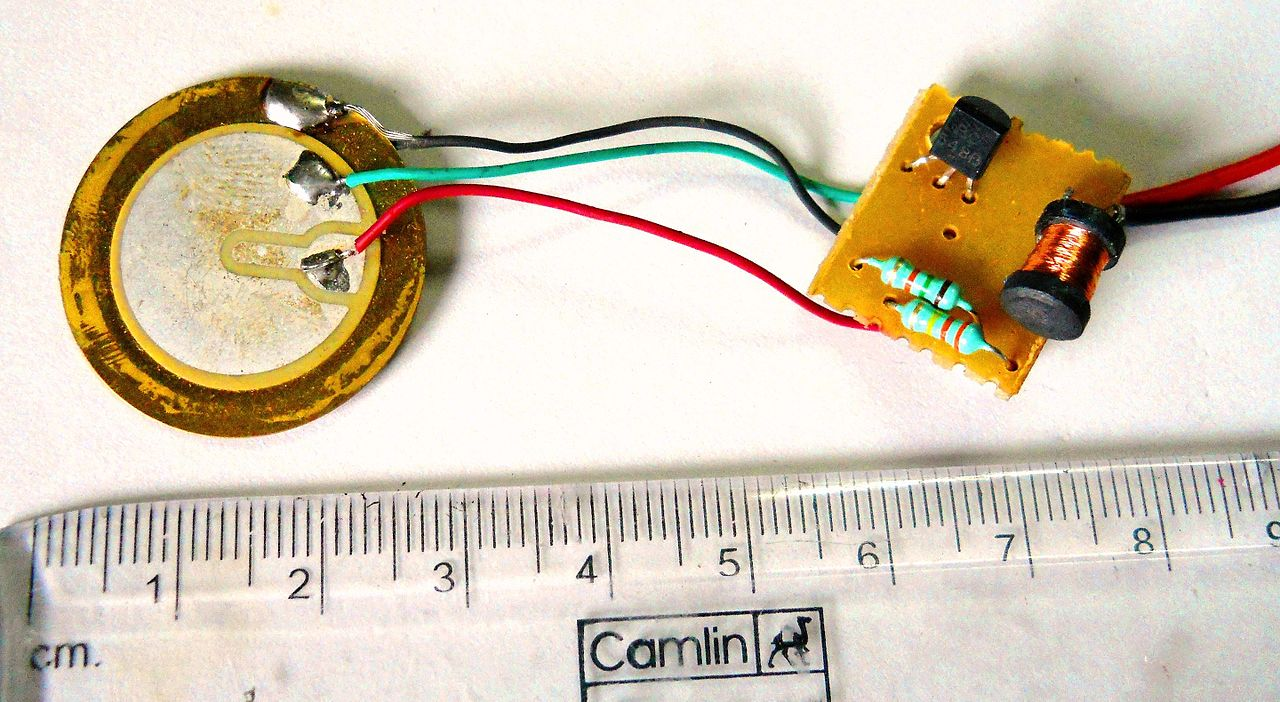
\includegraphics[width=0.7\textwidth]{internobuzzer}
  \caption{Interno di un buzzer \cite{wiki:internobuzzer}}
  \label{fig:internobuzzer}
\end{figure}

\subsection{Termometri}
Componente in grado di misurare la temperatura ambientale. Negli strumenti di misura possono essere usati per compensare le misurazioni
di componenti sensibili alle variazioni di temperatura nell'ambiente di utilizzo.
\subsection{Inclinometri a mercurio}
Particolari interruttori basati sulla gravità, i più semplici contengono una goccia di mercurio e due contatti elettrici, la cui chiusura dipende dalla
direzione della forza di gravità a cui è soggetto il componente: se la goccia viene spinta verso i contatti il circuito è chiuso, altrimenti rimane aperto.
Interruttore a mercurio in Figura~\ref{fig:mercuryswitch}.

\begin{figure}[h]
  \centering
  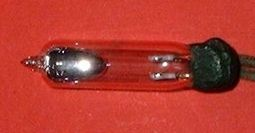
\includegraphics[width=0.5\textwidth]{mercuryswitch}
  \caption{Interruttore a mercurio in stato ``aperto" \cite{wiki:mercuryswitch}}
  \label{fig:mercuryswitch}
\end{figure}

%\todo{atrent: combinatore telefonico, suoneria}
\subsection{Disco combinatore}
Dispositivo generalmente trovato nei vecchi telefoni a disco (esempio in Figura~\ref{fig:siemenss62}) che consente di inviare un
treno di impulsi il cui numero varia in base all'angolo di rotazione a cui viene portato prima del rilascio.

\begin{figure}[h]
  \centering
  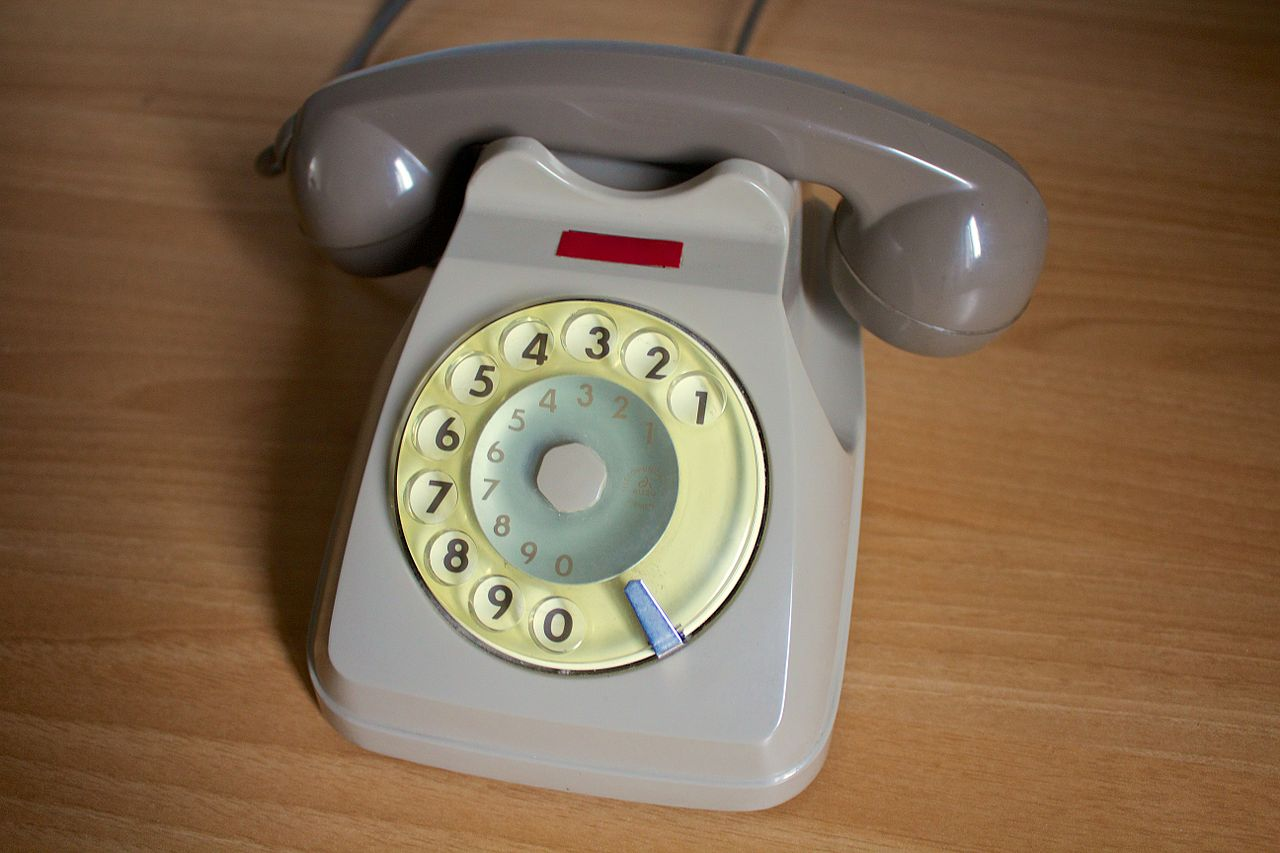
\includegraphics[width=0.7\textwidth]{siemenss62}
  \caption{Telefono Siemens S62, detto Bigrigio. Notare il disco combinatore \cite{wiki:siemenss62}}
  \label{fig:siemenss62}
\end{figure}

\subsection{Suonerie elettromeccaniche}
Anche queste generalmente trovate nei vecchi telefoni, se alimentate in corrente alternata con tensione intorno ai 110V
producono un deciso squillo. Sono ottime come segnalatori acustici.
%\todo{atrent: mi sa che la tensione delle suonerie telefoniche è intorno ai 50V (o 12V), fai check} %busolin: confermo 110V secondo Wikipedia
% https://it.wikipedia.org/wiki/Siemens_S62#Funzionamento

\chapter{Generalizzazione degli strumenti di misura}
%\todo{Sezione mapping componenti e interventi di modifica possibili}
In questo capitolo si tenterà di generalizzare le caratteristiche dei componenti degli strumenti di misura ai fini di associarle a componenti
software e tipi di dato.
%\todo{atrent: strada giusta! fai anche esempi pratici finali}

\section{Interruttori / Pulsanti}
Possono essere mappati a valori booleani (true/false). Collegabili da un capo a un terminale positivo o GND (in base a come viene letto
l'input) e dall'altro capo a un GPIO del microcontrollore. 
Possono essere utilizzati nel codice mediante la funzione digitalRead o come binary sensor su ESPHome\cite{esphomeio}:
\begin{lstlisting}[language=yaml]
binary_sensor:
  - platform: gpio
    pin: D2
    name: "Living Room Window"
    device_class: window
\end{lstlisting}
\noindent Esempio di schema di collegamento in Figura~\ref{fig:switchconnection}.
La connessione di un lato dello switch al polo positivo o negativo dell'alimentazione è una scelta architetturale da cui poi dipenderà
l'implementazione software.
Utilizzare un collegamento fra GND e il GPIO consente di sfruttare la resistenza interna di pull-up dell'ESP al fine di evitare il fenomeno
del ``float", per il quale a circuito aperto la rilevazione dello stato del pulsante alterna rapidamente tra ON e OFF a meno che il pin
di input sia ``tirato su" (o giù a segni invertiti).
In caso si volesse fare il contrario (fra 3.3V e il GPIO) per evitare floating è necessario aggiungere una resistenza esterna
di pull-down che collega il GPIO a GND e ``tiene giù" lo stato dell'input a meno che non sia chiuso il circuito.
Indipendentemente dal tipo di input, è possibile sia nel codice mediante un'inversione booleana sia in ESPHome mediante una flag
invertire la lettura qualora fosse necessario.

%\todo{atrent: spiega la dualità 3.3V/GND}

\begin{figure}[h]
  \centering
  \begin{circuitikz} \draw
    (0,0) to[cute open switch] (0,4)
   -- (4,4) node[above]{GPIO}
    to[twoport,t={ESP}] (4,0) node[below]{3.3V/GND}
    -- (0,0)
   
    ;
  \end{circuitikz}
  \caption{Schema collegamento switch all'ESP}
  \label{fig:switchconnection}
\end{figure}


\section{Commutatori a n posizioni}
Possono essere mappati in un programma a tipi \texttt{enum}, utilizzabili per selezionare tra un insieme di modalità o un insieme di valori
utilizzabili come parametro in un programma. Ad esempio un commutatore a 7 posti può essere utilizzato per selezionare un giorno della
settimana.

Per evitare di occupare tanti pin del microcontrollore quante sono le possibili posizioni di un commutatore, è possibile convertirlo in un
partitore di tensione mediante l'ausilio di resistenze tutte uguali con valore totale intorno ai 10k$\Omega$,
collegate come da esempio in Figura~\ref{fig:commutatoreprimadopo} e \ref{fig:rotaryconnection},
ottenendo una sorta di potenziometro che invece di variare nel continuo assume valori in step regolari tra il minimo e il massimo
dell'ingresso, che possono essere agevolmente distinti e interpretati come valori discreti.

Si considera una resistenza totale di 10k$\Omega$ al fine di mantenere un flusso di corrente tra 3.3V e GND
quanto più piccolo possibile, per non influire eccessivamente né sul consumo di corrente né sulla temperatura dei componenti.
Una resistenza totale di 10000$\Omega$ a 3.3V, per la legge di Ohm ($V = R \times I$ e quindi $I = V / R$) produrrà un flusso
costante di corrente di appena 0.33$mA$.

Per la lettura valgono le considerazioni fatte sui potenziometri, bisognerà
poi via software fare dei calcoli per riconoscere gli step e utilizzarli a dovere nel codice.

\begin{figure}[h]
  \centering
  \subfloat[Prima]{{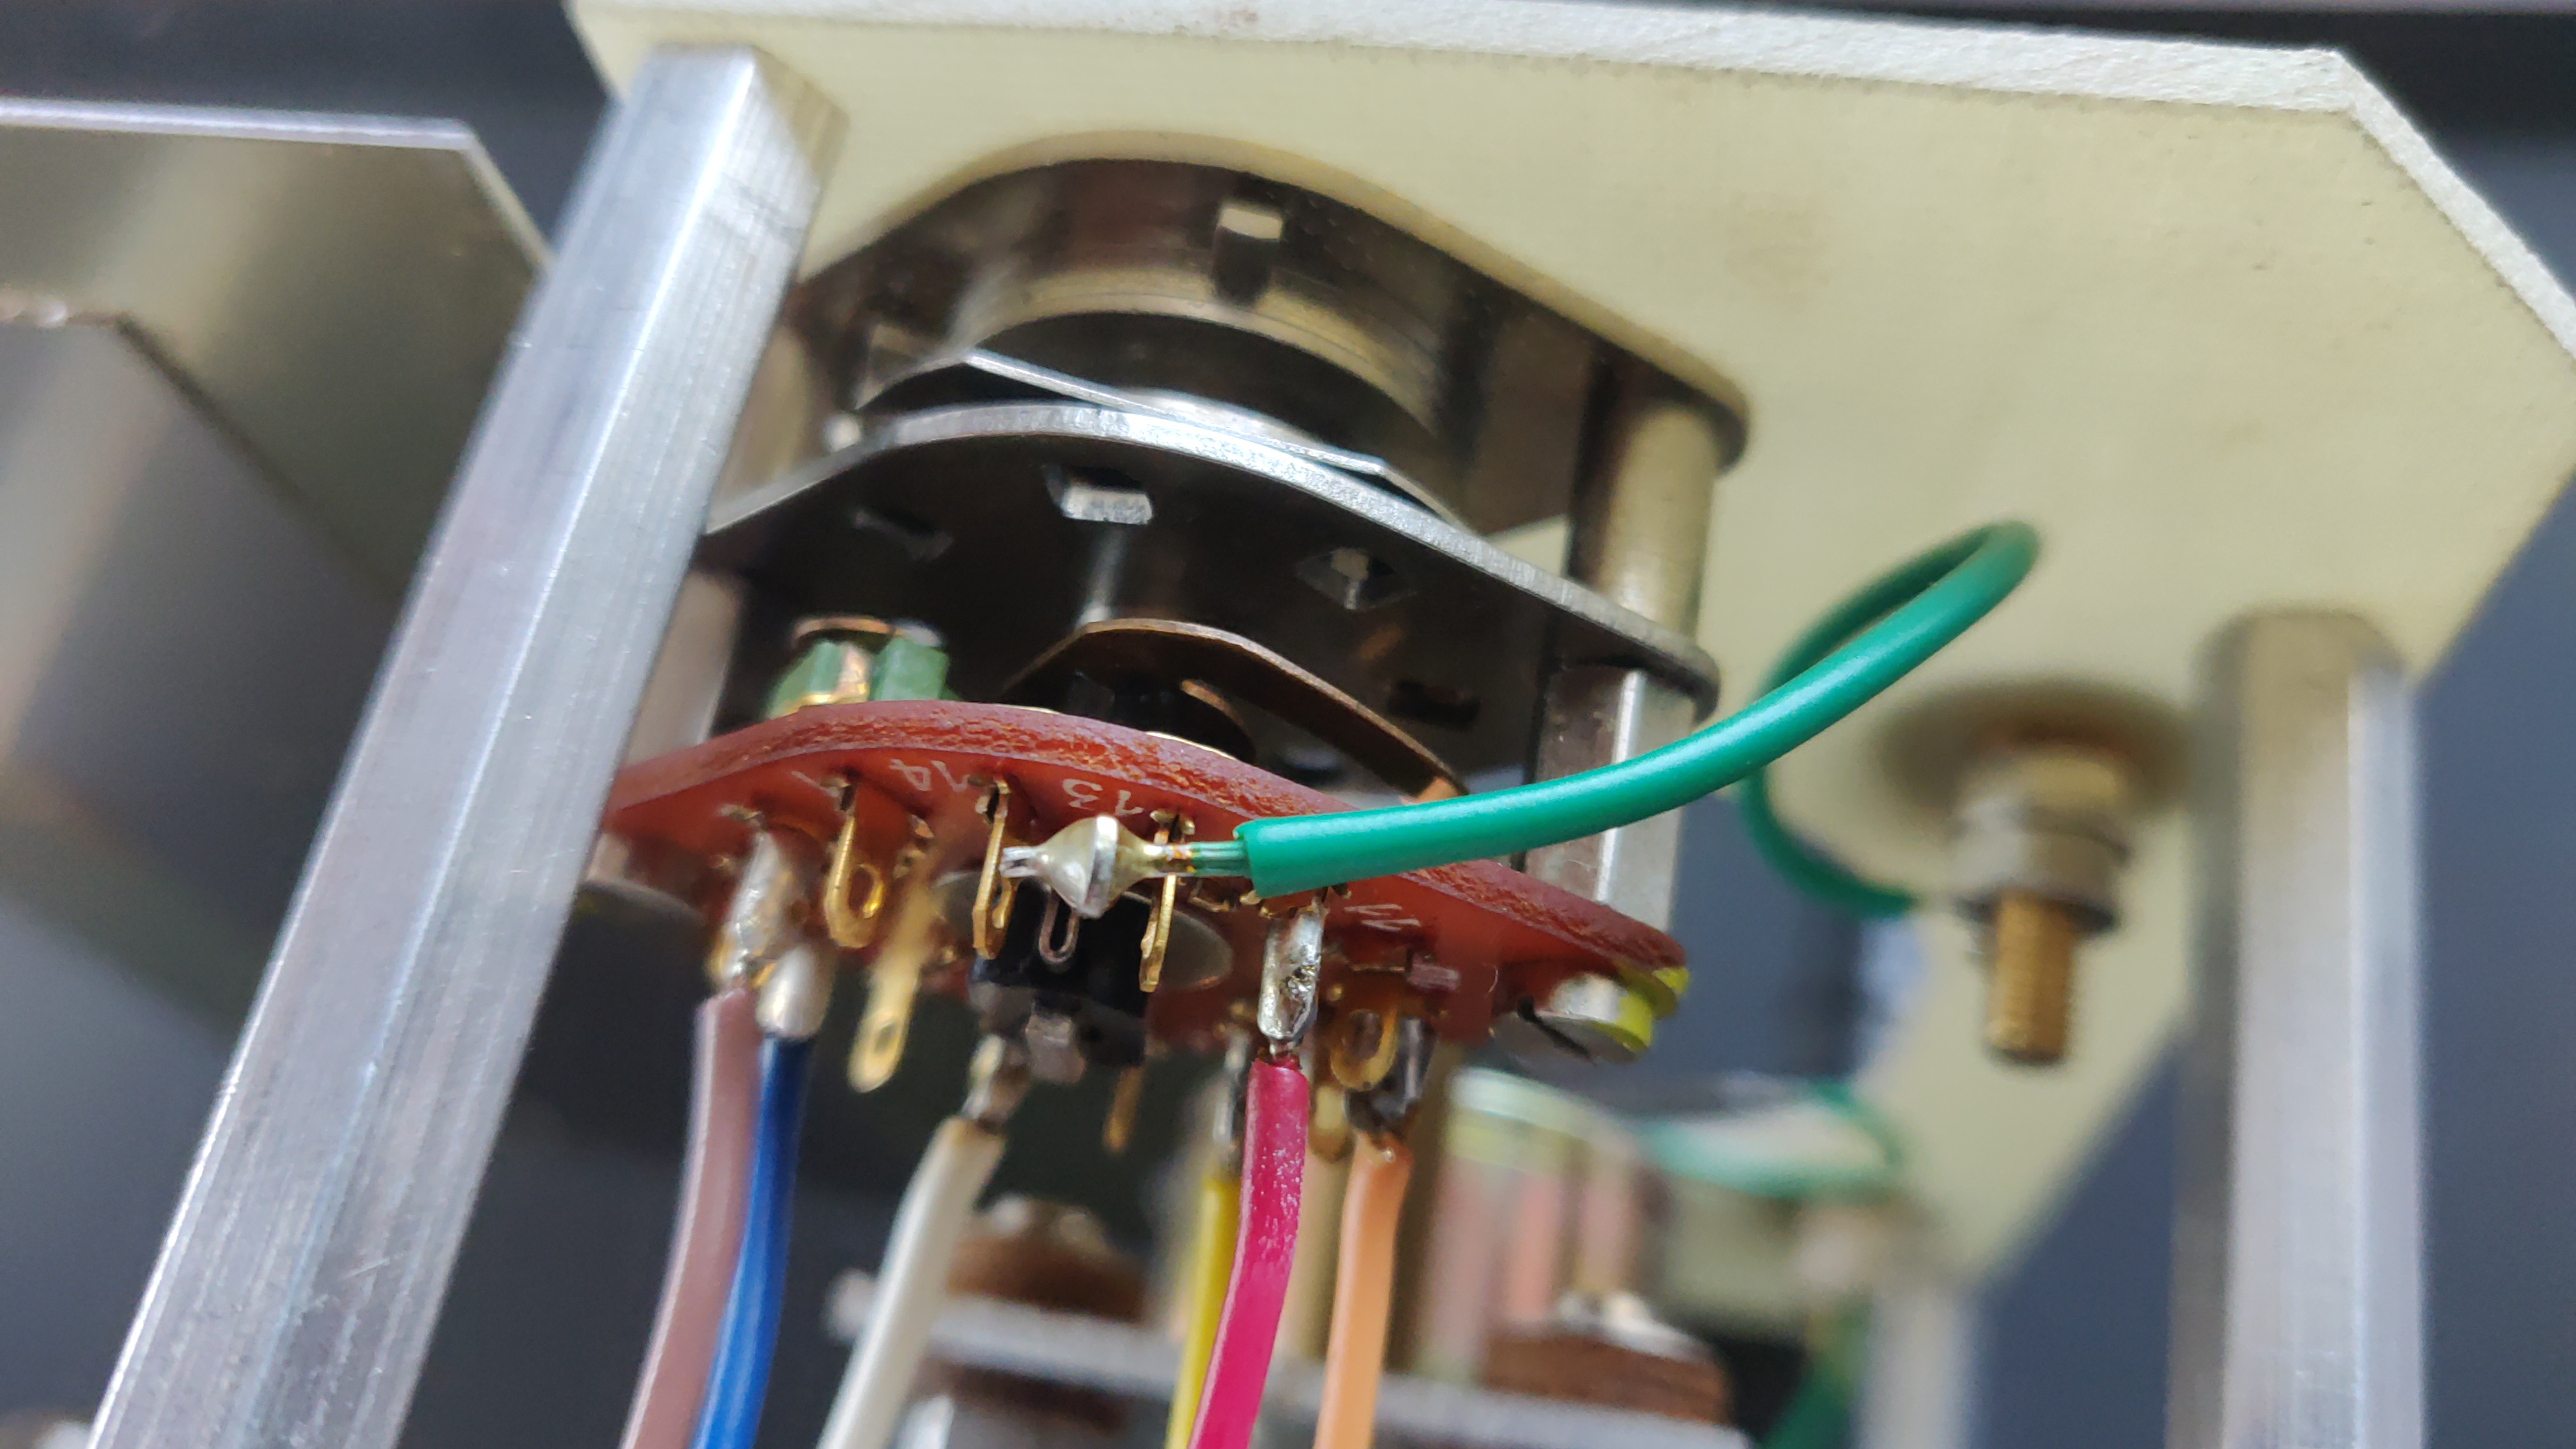
\includegraphics[height=3.5cm]{commutatoreStock}}}
  \enspace
  \subfloat[Dopo]{{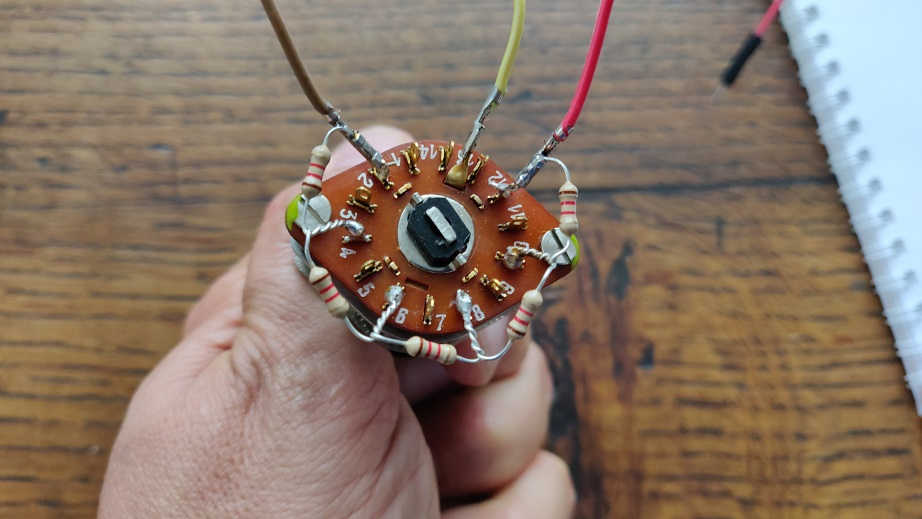
\includegraphics[height=3.5cm]{commutatorePartitore}}}
  \caption{Dettaglio commutatore prima e dopo la modifica come partitore}
  \label{fig:commutatoreprimadopo}
\end{figure}

\begin{figure}[h]
  \centering
  \begin{circuitikz} \draw
    (0,0) to[twoport,t={ESP},  n=esp] (0,6)

    (2,3)  node[rotary switch  -=4 in 90 wiper 15, anchor=in](SW){}
    (SW.in) to[short] (1.2,3) node[above]{Analog} node[below]{IN} to (esp)
   

    (4,6) to[R=R1] (4,4) to[R=R2] (4,2) to[R=R3] (4,0) 
    (0,6) -- (4,6)
    (0,0) -- (4,0)

    (SW.out 1) to[short, -*] (4,6) node[above]{3.3V}
    (SW.out 2) to[short, -*] (4,4)
    (SW.out 3) to[short, -*] (4,2)
    (SW.out 4) to[short, -*] (4,0)  node[below]{GND}
  ;
  \end{circuitikz}
  \caption{Schema collegamento commutatore modificato all'ESP. Le tre resistenze hanno lo stesso valore}
  \label{fig:rotaryconnection}
\end{figure}

\todo{atrent: a onor del vero le resistenze possono anche essere diverse, ma poi i conti sono meno banali (software intendo)}

%\todo{atrent: spiega un minimo la scelta delle resistenze, perché 10KOhm, legge di Ohm...}

\section{Potenziometri}
Possono essere mappati a valori aventi intervallo arbitrario, con una precisione limitata dalla risoluzione del convertitore analogico-digitale
integrato nel microcontrollore. Per poter leggere l'output è necessario collegarli a un GPIO che supporta la lettura di segnali analogici
e nel codice utilizzare la funzione analogRead. Su ESPHome è necessario usare sensori di tipo adc\cite{esphomeio}:
\begin{lstlisting}[language=yaml]
sensor:
  - platform: adc
    pin: A0
    name: "Living Room Brightness"
\end{lstlisting}
\noindent Esempio di collegamento in Figura~\ref{fig:potconnection}

\begin{figure}[h]
  \centering
  \begin{circuitikz} \draw
    (0,4) to[potentiometer, n=pot] (0,0)
    (0,4) to[short] (4,4) node[above]{3.3V}
    to[twoport,t={ESP}, n=esp] (4,0) node[below]{GND}
    -- (0,0)
    (pot.wiper) to[short] (2.5,2) node[above]{Analog} node[below]{IN} to (esp)
  ;
  \end{circuitikz}
  \caption{Schema collegamento potenziometro all'ESP}
  \label{fig:potconnection}
\end{figure}

\section{Connettori multipli}
Alcuni strumenti dispongono di più ingressi per le sonde di misura, adatti a connettori a banana o non standard, specifici alle
diverse modalità di misura e/o i diversi fondoscala tra cui scegliere. Possono essere utilizzati come selettori a livello software in base a
quali degli ingressi vengono ponticellati, in maniera simile alle connessioni tra utenze telefoniche nei vecchi centralini o agli spinotti per
gli scambi di lettere presenti sulla macchina Enigma. Si riporta un esempio in Figura~\ref{fig:connettorimultipli}.

\begin{figure}[h]
  \centering
  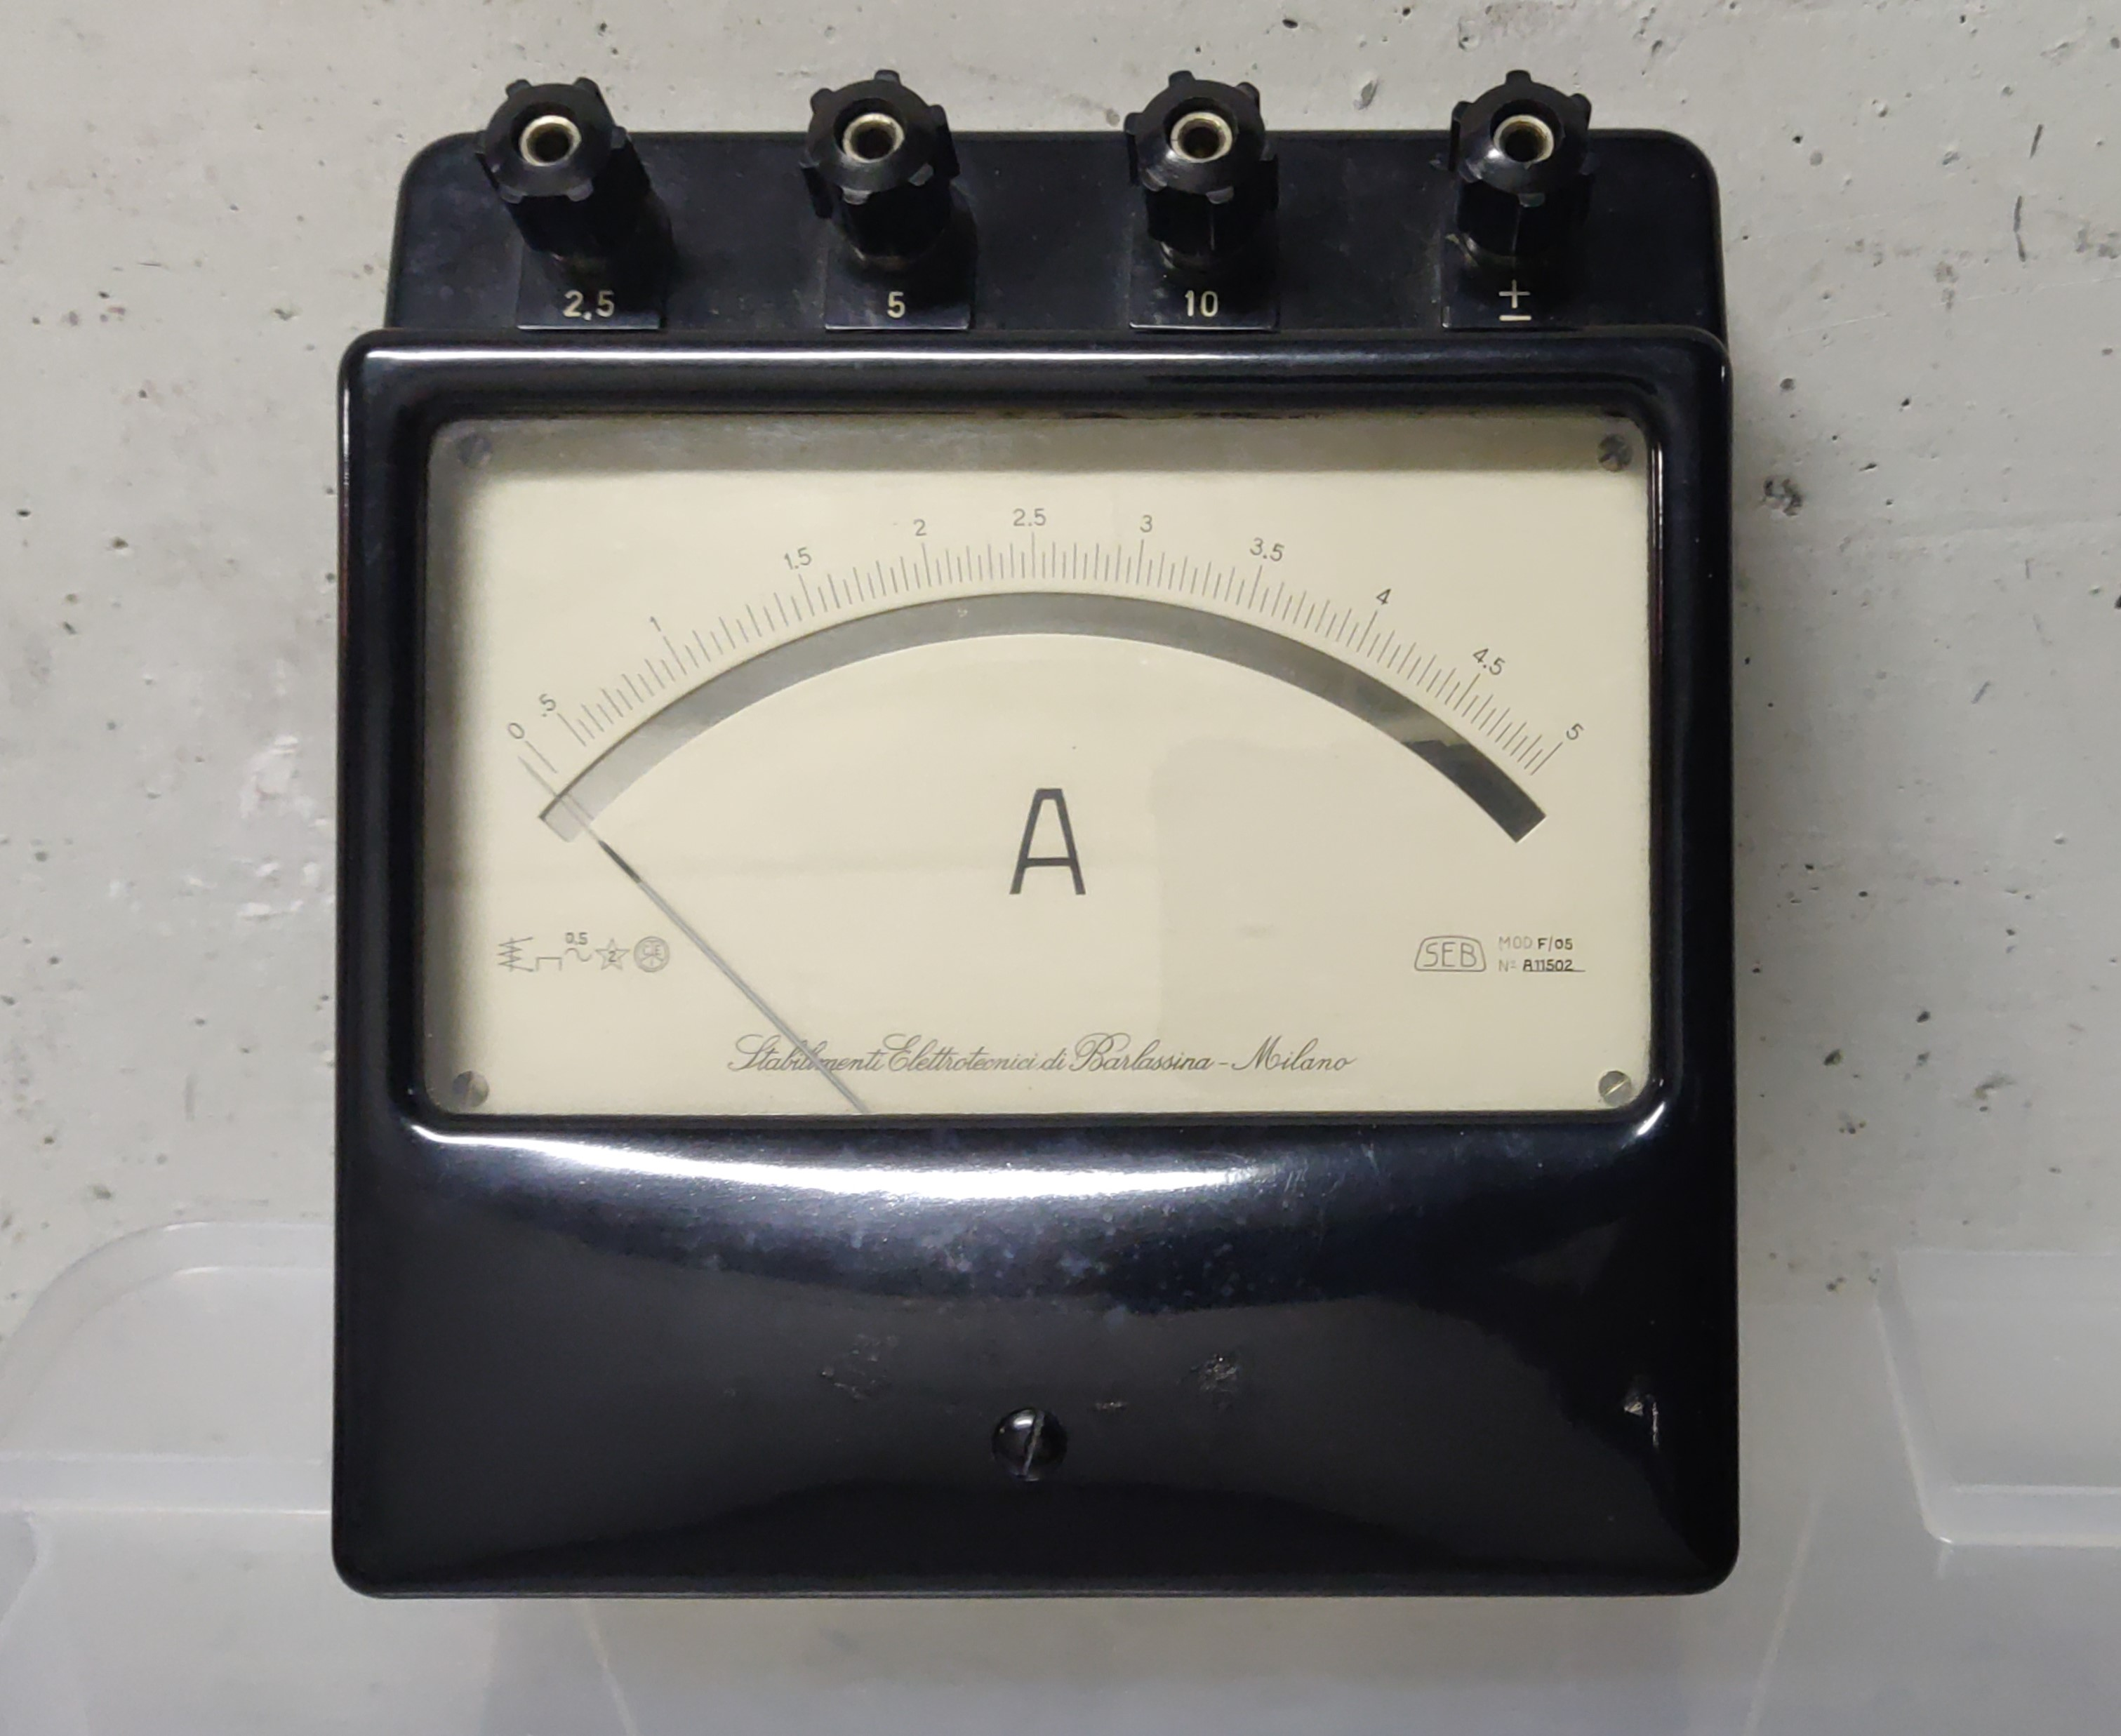
\includegraphics[width=0.8\textwidth]{connettorimultipli}
  \caption{Amperometro con connettori separati in base alla scala}
  \label{fig:connettorimultipli}
\end{figure}

\section{Lampadine}
Possono essere utilizzate per rappresentare uno stato in maniera binaria o comunicando mediante dei pattern di lampeggi e in alcuni
casi anche di colore.
In genere con i sistemi embedded si adoperano i LED al posto delle lampadine a incandescenza, in quanto possono essere pilotati
direttamente dai pin del microcontrollore, salvo eventuali resistenze in serie per ridurre il flusso di corrente.
Nel codice di Arduino un LED può essere pilotato mediante una digitalWrite per funzionamento on/off o una analogWrite per
intensità variabili mediante PWM (in maniera simile a come si è fatto con l'ago dello strumento per il prototipo).
In ESPHome si può utilizzare un componente di tipo light, il più semplice è quello binario\cite{esphomeio}:
\begin{lstlisting}[language=yaml]
light:
  - platform: binary
    name: "Desk Lamp"
    output: light_output

output:
  - id: light_output
    platform: gpio
    pin: GPIO16
\end{lstlisting}
%\todo{atrent: in realtà non solo uno stato binario, se vedi lo status led di esphome c'è un codice lampeggi semantico (come c'è ancora un codice buzz per il BIOS dei PC (mi pare ad esempio 5 beep errore ram, ecc.)}

Esistono molti altri tipi di componenti light, tra cui PWM monocromatici ed RGB, sia con apposito circuito integrato di controllo (come
quello basato su driver WS2801 utilizzato nel prototipo) che a collegamento individuale dei singoli colori.



\section{Buzzer/Altoparlanti}
Possono essere usati per dare indicazioni audio, ad esempio in caso di errore. I buzzer possono solitamente essere pilotati direttamente
dal microcontrollore, mentre gli altoparlanti spesso richiedono un amplificatore di potenza.
Il funzionamento dal punto di vista software dipende dal tipo di buzzer utilizzato: un buzzer attivo contiene al suo interno un oscillatore
e quindi genererà un beep mentre è alimentato. Un buzzer passivo si comporta in maniera simile a un altoparlante (in effetti ne è un tipo
particolare) in quanto ha bisogno di un segnale audio in ingresso.
Attraverso ESPHome è possibile riprodurre delle semplici melodie con buzzer passivi utilizzando il componente rtttl. Si riporta a seguito
l'esempio di configurazione di un componente buzzer che riproduce il tema di Mission Impossible\cite{esphomeio}:
\begin{lstlisting}[language=yaml]
output:
  - platform: ledc
    pin: GPIO22
    id: rtttl_out

rtttl:
  output: rtttl_out

on_<event>:
  then:
    - rtttl.play: 'MissionImp:d=16,o=6,b=95:32d,32d#,32d,32d#,32d,32d#,32d,32d#,32d,32d,32d#,32e,32f,32f#,32g,g,8p,g,8p,a#,p,c7,p,g,8p,g,8p,f,p,f#,p,g,8p,g,8p,a#,p,c7,p,g,8p,g,8p,f,p,f#,p,a#,g,2d,32p,a#,g,2c#,32p,a#,g,2c,a#5,8c,2p,32p,a#5,g5,2f#,32p,a#5,g5,2f,32p,a#5,g5,2e,d#,8d'
\end{lstlisting}
\section{Inclinometri a mercurio}
Ai fini implementativi hanno un funzionamento al pari degli interruttori/pulsanti. L'unica differenza sta nel principio fisico di funzionamento
e quindi nel significato che si può dare all'output nel codice.

\section{Disco combinatore}
Come descritto precedentemente, questo tipo di dispositivo produce una sequenza di impulsi che vanno letti e contati. ESPHome mette
a disposizione un componente che consente di eseguire questo tipo di lettura in maniera semplice:
\begin{lstlisting}[language=yaml]
sensor:
  - platform: pulse_counter
    pin: 12
    name: "Pulse Counter"
\end{lstlisting}

\chapter{Guida alla trasformazione degli strumenti vintage}
%\todo{Sezione guida alla conversione vera e propria che fa riferimenti alla sezione precedente}

%\todo{atrent: manca una trattazione di come è fatto e come funziona lo strumento ad ago (che sarà il più frequente oggetto di visualizzazione), spiega bene la sua architettura, wikipedia is your friend}


%\todo{atrent: tenterei anche una panoramica storica degli strumenti di ``visualizzazione'' (occhi magici, elettrofori, dekatron, oscilloscopi, ...) dando idee su come si potrebbero usare per datafisicalizzare}

\section{Introduzione}
Una volta appurate le caratteristiche degli strumenti e i possibili utilizzi dei componenti che vi si possono trovare, è opportuno discutere
della loro conversione.


\section{Interventi}
\subsection{Intervento minimale}
Il metodo più semplice per ottenere un oggetto funzionante è quello di collegare il GPIO del microcontrollore settato come output
e GND rispettivamente al terminale positivo e negativo dello strumento di misura in modalità voltmetro. Se la tensione in uscita massima
coincide con il fondoscala dello strumento di misura questo è sufficiente, altrimenti è necessario ridurla via software oppure
utilizzare un partitore di tensione o un potenziometro. Nel caso in cui la tensione in uscita massima del microcontrollore sia inferiore
ad ogni possibile fondoscala dello strumento di misura, questo metodo non è attuabile. Esempio di intervento minimale in
Figura~\ref{fig:interventominimale}. Notare il cavo collegato ai terminali: il microcontrollore è esterno
e i commutatori devono rimanere nella posizione rappresentata per consentire un corretto funzionamento.

\begin{figure}[h]
  \centering
  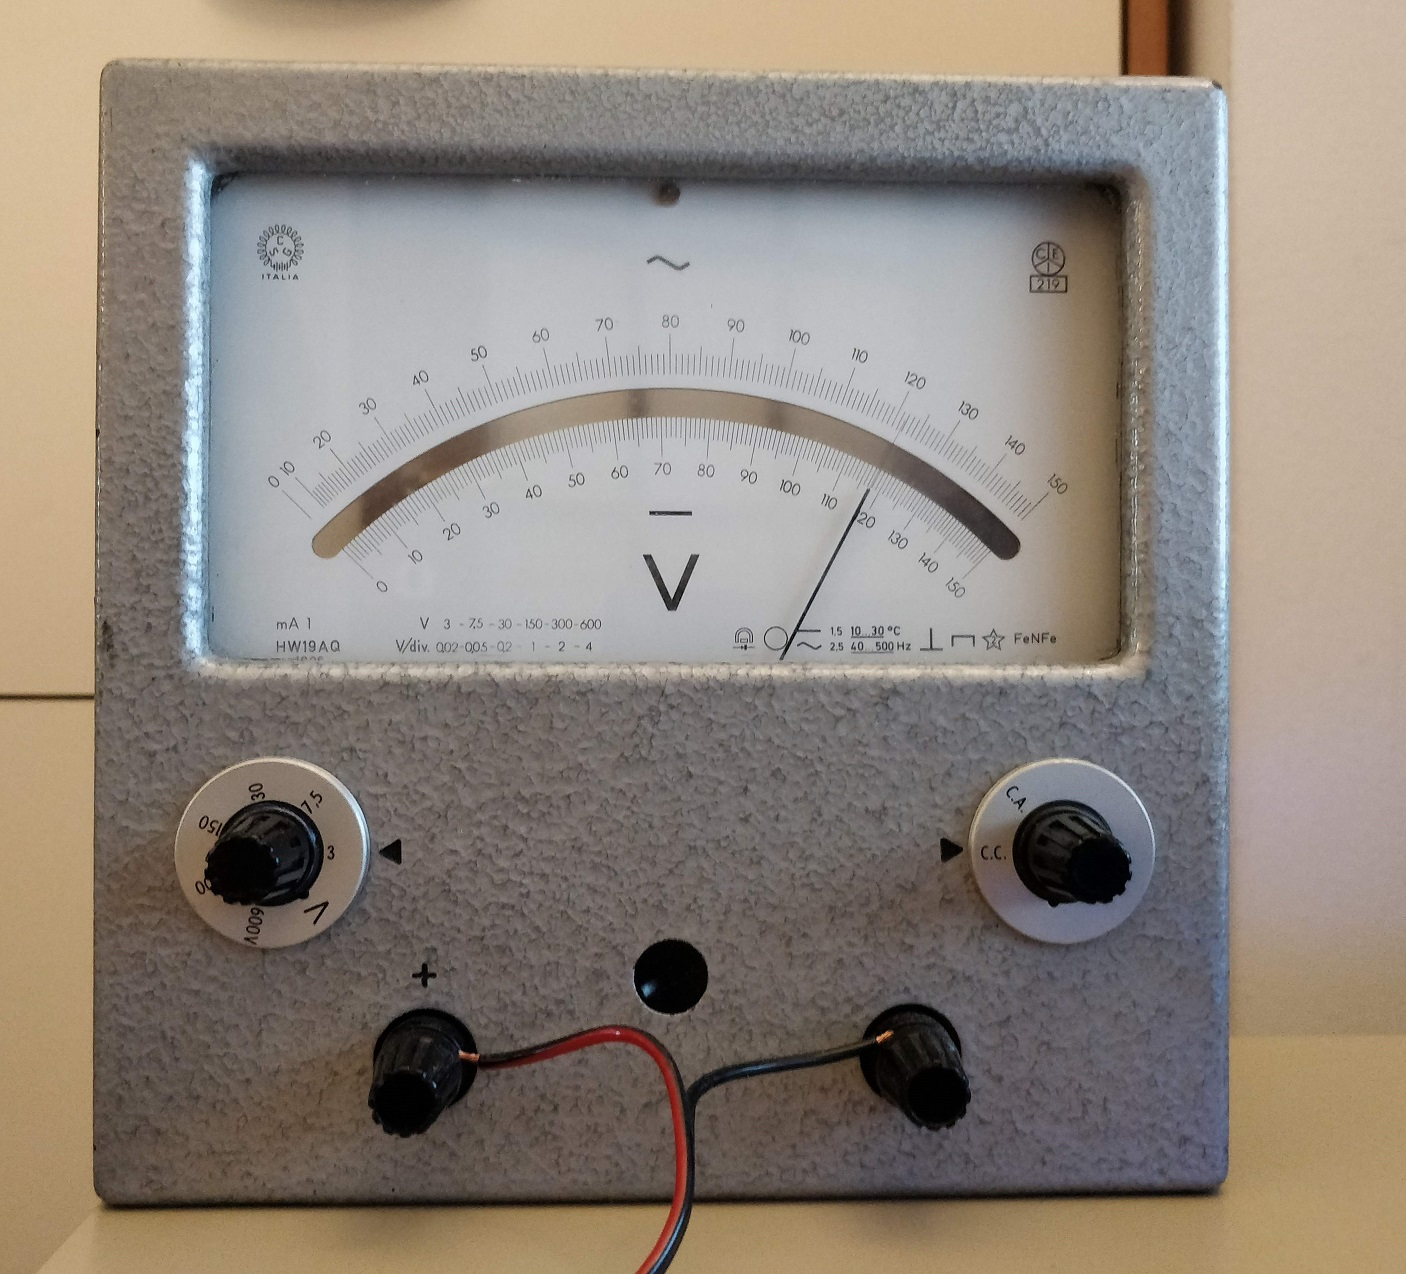
\includegraphics[width=0.8\textwidth]{interventominimale}
  \caption{Esempio di intervento minimale}
  \label{fig:interventominimale}
\end{figure}

\subsection{Intervento approfondito}
Un metodo più invasivo ma più pulito consiste nel modificare la struttura interna dello strumento di misura, collegandosi ai capi dello
strumento interno vero e proprio bypassando selettore di modalità/fondoscala.
Se non si vuole rimpiazzare la resistenza interna valgono le stesse osservazioni fatte poc'anzi sui fondoscala: è necessario che
esista una modalità con fondoscala minore o uguale alla tensione di uscita massima del microcontrollore, altrimenti sarà necessario
utilizzare una resistenza più piccola di quella/e già presente/i.
In generale vale la pena di rimuovere la scheda resistenze e utilizzare solamente una resistenza di valore adatto.

Una volta aperto lo strumento (ed eventualmente rimosse circuiterie varie non necessarie) si possono incontrare tutta una serie
di componenti tra cui quelli descritti nel capitolo precedente. Alcuni saranno adattabili all'utilizzo con microcontrollori mentre altri no.

Esiste un caso in cui, nonostante la rimozione delle resistenze di taratura, la sensibilità dello strumento rimane più bassa di quanto
desiderato e la tensione massima che può emettere il microcontrollore non basta per arrivare a fondoscala. In questo caso le alternative
sarebbero adoperare un survoltore per raggiungere la tensione necessaria oppure rinunciare e provare con un altro strumento.

Questo livello di modifica consente di integrare (a condizione che ci sia spazio, gli strumenti in Figura~\ref{fig:strumentiago} sono
quasi tutti adatti) il microcontrollore all'interno dello strumento in modo da ottenere un sistema composto da un solo oggetto.
Se si ha la facoltà di inserire una batteria diventa anche incredibilmente discreto e di più facile posizionamento, anche dove è
scomodo portare una fonte di alimentazione.

\todo{atrent: qui avrei messo almeno anche la foto della scheda resistenze e mi sarei ricollegato all'uso del commutatore convertito, insomma avrei spiegato un po' più nel dettaglio tutte le operazioni fatte, hai tutte le foto interne a disposizione...}

\subsection{Interventi aggiuntivi}
Ulteriori possibili modifiche meno banali includono l'aggiunta di elementi decorativi e/o funzionali quali luci, bottoni e altoparlanti
per ampliare le possibilità di utilizzo. Un'altra possibilità di modifica ove possibile è la sostituzione dell'etichetta dietro all'ago per adattare
la scala rappresentata alla vera scala dei dati (a condizione che questa rimanga fissa). Adoperando un display e-paper si potrebbe
adattare dinamicamente la scala rappresentata dallo strumento senza più bisogno di interventi fisici.

Esempio di strumento dopo modifiche avanzate in Figura~\ref{fig:interventocompleto}:
è stato sostituito il terminale sinistro con un connettore USB da pannello ai fini di interfacciarsi con il microcontrollore e alimentarlo.
Il terminale destro è stato sostituito con un indicatore LED, il commutatore
destro con un pulsante e all'interno è stato posizionato un buzzer che consente di riprodurre dei suoni insieme a un LED RGB.


%\todo{atrent: c'è anche un led RGB (WS2812B)}

%\todo{atrent: aggiungo screenshot HA}

\begin{figure}[h]
  \centering
  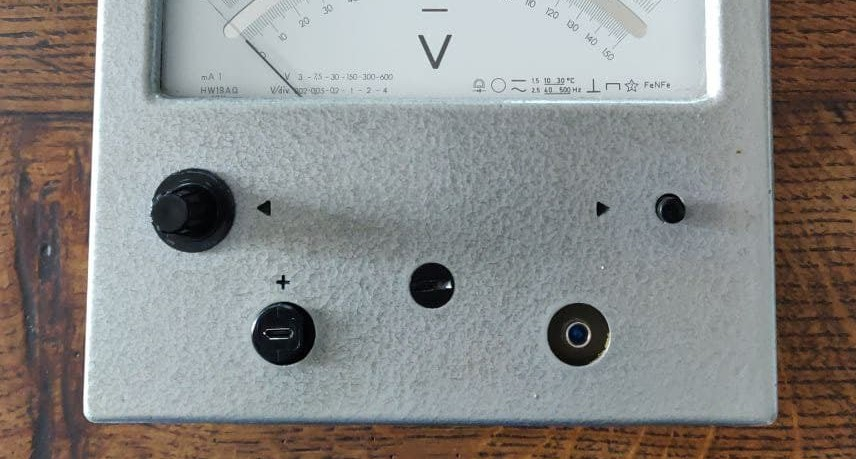
\includegraphics[width=0.9\textwidth]{interventocompleto}
  \caption{Esempio di strumento dopo modifiche avanzate}
  \label{fig:interventocompleto}
\end{figure}

\chapter{Il prototipo - IoTDial}
Questo capitolo tratterà dell'implementazione delle varie feature del prototipo realizzato durante il tirocinio, chiamato IoTDial,
il loro utilizzo e alcune osservazioni al riguardo.

Il prototipo era inizialmente molto semplice dal punto di vista hardware: consisteva in un voltmetro analogico ad ago impostato con
fondoscala a 3V e un WeMos D1 mini basato su ESP8266. Il terminale positivo del voltmetro era connesso a un GPIO dell'ESP,
mentre il terminale negativo a GND.

Successivamente sono stati eseguiti maggiori interventi fisici fino ad arrivare alla situazione visibile in Figura~\ref{fig:interventocompleto}
e descritta nella corrispondente sezione, con il microcontrollore inserito all'interno della scocca dello strumento e alcune modifiche estetiche
e funzionali.

\section{Contesti d'uso}
\subsection{Ruoli}
Prima di parlare del delle modalità operative di IoTDial è il caso di soffermarsi su chi vi può interagire:

%\todo{atrent: diventa una bullet list, meglio}
\begin{itemize}
  \item Sviluppatore:
È in grado di apportare modifiche al codice sorgente. Può aggiungere, rimuovere e  modificare funzionalità del programma
e apportare modifiche dirette ai file di configurazione.
  \item Utente esperto:
Conosce le API ed è in grado di comprendere il formato dei dati che restituiscono. Gli è sufficiente un'interfaccia anche spartana
per selezionare la sorgente dei dati e il campo specifico che vuole rappresentato.
  \item Utente inesperto:
Non conosce le API né il formato JSON, è possibile che abbia anche una limitata conoscenza del mondo informatico:
ha bisogno di un prodotto già pronto che richieda la minima configurazione possibile e questa
deve essere particolarmente intuitiva. 
\end{itemize}
%\todo{atrent: questi sono i ruoli, mancano gli use case veri e propri (parlando formalmente, faccio riferimento a UML)}

\subsection{Use case}

\subsubsection{API/Standalone}
Questa modalità di operazione si basa sull'esecuzione ad intervalli di tempo configurabili di richieste HTTP o HTTPS ad API REST
e sulla conversione del risultato in una tensione di uscita, avendo in più le funzionalità descritte successivamente nella sezione
sulla implementazione software.
È considerata ``standalone" in quanto fornita una connessione di rete funziona in autonomia.

Gli interventi al codice richiedono uno sviluppatore, la configurazione della fonte API e la gestione dei multipli file di configurazione
mediante le interfacce messe a disposizione sono nelle corde di un utente esperto mentre per l'utente inesperto risulta necessario
fornire un prodotto già pronto; potrebbe giusto configurare la rete WiFi mediante l'access point integrato e il web form e
selezionare tra fonti di dati o configurazioni diverse mediante interazione con un commutatore fisico.

\subsubsection{Smart Home/Passivo}
%\todo{rivedere}
Questa modalità si basa sulla piattaforma ESPHome ed è considerata ``passiva" in quanto l'idea di base prevede un'integrazione
e dipendenza con altri oggetti all'interno o all'esterno della rete locale per funzionare a dovere, specialmente per l'interpretazione
dei dati dei componenti aggiuntivi connessi.
Esiste il modo di rendere un sistema ESPHome completamente autonomo mediante l'utilizzo di procedure interne ma non verrà
approfondito in questa sede.
In questo caso, uno sviluppatore è richiesto per adattare il file di configurazione di ESPHome ai vari dispositivi collegati,
specialmente per quanto riguarda automatismi interni indipendenti da sistemi di home automation.
Una configurazione totalmente ``passiva" e relegata all'interazione con sistemi di home automation, invece, può essere effettuata
anche da un utente esperto, vista la semplicità d'uso delle configurazioni di base di ESPHome e delle interfacce dei sistemi con cui
si andrà a interfacciare.
Ancora una volta per l'utente inesperto è necessario fornire un dispositivo già configurato e pronto all'uso, al netto di
configurazioni della rete WiFi con un meccanismo simile a quello implementato nella modalità API.


\section{Implementazione modalità API}
La parte software della modalità API (o standalone) è stata realizzata utilizzando il linguaggio di programmazione di Arduino, esteso
all'utilizzo con ESP8266, e con l'aiuto di numerose librerie.
Come IDE è stato usato Visual Studio Code con l'estensione PlatformIO, la quale permette di specificare le dipendenze direttamente
in file di configurazione e di scaricare automaticamente le librerie necessarie per ogni progetto.

\subsection{PWM}
Il principio di base che permette di produrre una tensione variabile da parte di un sistema digitale è la Pulse-Width Modulation.
Ciò consente di controllare finemente la posizione dell'ago del voltmetro via software.

\subsection{Richieste API}
Il primo passo verso la fisicalizzazione dei dati è stato quello di ottenerli, mediante richieste ad API REST in locale o su Internet.
Per questo è stata utilizzata la libreria \texttt{ESP8266HTTPClient}.


\begin{lstlisting}[language=cpp]
bool begin;
if (use_https) {
  begin = http.begin(ssl_client, apiUrl);
  Serial.print("[HTTPS] ");
} else {
  begin = http.begin(client, apiUrl);
  Serial.print("[HTTP] ");
}

Serial.print("begin... ");
Serial.println("URL: " + apiUrl);
\end{lstlisting}

Le richieste HTTP hanno funzionato fin da subito, per HTTPS c'è stato più da lavorare in quanto non erano eccessivamente
documentate e tutte le soluzioni trovate online prevedevano l'utilizzo di stringhe per memorizzare intere risposte, che per via
della limitata disponibilità di memoria dell'ESP non è sempre una soluzione adeguata.
Un'alternativa fornita dalla libreria è quella di utilizzo di uno stream, per poter leggere dalla risposta un byte alla volta senza doverla
memorizzare per intero, potendo ignorare le parti non necessarie. Questo meccanismo però è di facile utilizzo solo finché ci si limita a
HTTP. Per HTTPS la funzione per estrarre lo stream della risposta, secondo la documentazione della libreria, non è supportata.
Per questo motivo è stato utilizzato come stream direttamente il BearSSL::WiFiClientSecure referenziato dalla connessione, impostato in
modalità insicura (senza la verifica della fingerprint), che però non sempre presenta un output  ``pulito" della risposta ma essa potrebbe
essere preceduta da una linea contenente (presumibilmente) la lunghezza in byte della risposta, che va eliminata prima di poter
passare lo stream al parser JSON.

Si riporta la sezione di codice che chiama un metodo di callback il quale accetta uno stream come argomento. Notare che per una richiesta
HTTP è utilizzato il metodo getStream messo a disposizione dalla libreria, mentre per HTTPS viene passato direttamente il client WiFi.
\begin{lstlisting}[language=cpp]
if (httpCode == HTTP_CODE_OK) {
  if (use_https) {
    callback(ssl_client);
  } else {
    callback(http.getStream());
  }
}
\end{lstlisting}

\subsection{Risposte JSON}
La quasi totalità delle API mette a disposizione risposte contenenti dati in formato JSON (JavaScript Object Notation). È stata quindi
utilizzata la libreria \texttt{ArduinoJson} per la deserializzazione e la scelta del campo da estrarre.
JSON è stato successivamente usato anche come formato per la serializzazione e deserializzazione delle impostazioni da salvare sulla
memoria flash dell'ESP per permetterne la persistenza anche a seguito di perdite di tensione.

Segue una porzione di codice della callback che evidenzia l'utilizzo di uno stream con buffer da 64 byte ai fini di un miglioramento delle
performance, la deserializzazione del filtro e la ``pulizia" dello stream nel caso in cui si usi HTTPS ed esso contenga caratteri iniziali
diversi dalle parentesi.
\begin{lstlisting}[language=cpp]
void stream_callback(Stream &stream) {
  ReadBufferingStream rbs(stream, 64);
  StaticJsonDocument<200> filter;
  deserializeJson(filter, filterJSON);
  Serial.println("--- Start of text excluded from stream ---");
  while (rbs.available() && char(rbs.peek()) != '{' && char(rbs.peek()) != '[') {
    Serial.print(char(rbs.read()));
  }
  Serial.println("---  End of text excluded from stream  ---");
  DynamicJsonDocument doc(2000);
  deserializeJson(doc, rbs, DeserializationOption::Filter(filter));
\end{lstlisting}

\subsection{Approfondimento su filtro JSON e path}
Il centro del funzionamento della modalità API e la sua adattabilità all'utilizzo di fonti dati diverse risiede nei campi
filterJSON e path.
\texttt{filterJSON} consente di evitare che tutta la risposta delle API venga salvata in memoria. Viene quindi scartato ogni campo che non
appaia come placeholder all'interno della stringa, ad esempio:
\texttt{"\{Lines: [\{WaitMessage: true\}]\}"} consente di mantenere
in memoria solo il campo con chiave WaitMessage di ogni elemento contenuto nell'array avente chiave Lines. Questa funzionalità è
implementata e ben documentata nella libreria \texttt{ArduinoJSON}.~\cite{arduinojsonfiltering}

Questo filtro non è sufficiente come indicatore del campo desiderato, in quanto il documento JSON salvato in memoria conterrà comunque
tutta la gerarchia e per come funzionano i placeholder sugli array non è neanche detto che ci sia in totale un solo campo con un valore
assegnato.
Per questo motivo è stato aggiunto il campo \texttt{path} alla configurazione e implementato nel codice un metodo di parsing specifico.
Questa stringa, nel programma, viene interpretata token per token prendendo gli slash come separatori e usata per esplorare
la gerarchia del documento JSON. Un token completamente numerico viene visto come indice di un array, altrimenti come chiave da
cercare all'interno di un oggetto.

Per fare un esempio coerente con il precedente: \texttt{"Lines/0/WaitMessage"} verrà approcciato nel seguente modo:
\begin{itemize}
  \item Interpretare la radice come un oggetto, cercare la chiave \texttt{Lines} e spostarvisi all'interno;
  \item Interpretare il successivo livello come un array, estrarre l'elemento in posizione 0 e spostarvisi all'interno;
  \item Interpretare il successivo livello come un oggetto, cercare la chiave \texttt{WaitMessage} e spostarvisi all'interno.
\end{itemize}
A questo punto, finita la stringa, il programma assumerà di trovarsi dinnanzi a un campo interpretabile come numerico (tollera molto,
ad esempio la stringa ``123aaa" verrà interpretata come 123.00) e lo estrarrà come risultato. %excursus JsonVariant?

Questo approccio, grazie alla cura con cui è implementata la libreria \texttt{ArduinoJson}, è molto tollerante a errori o inesattezze.
Se nel JSON non fosse presente un campo desiderato durante il parsing della path, così come se non fosse possibile la conversione
da stringa a numero presente subito dopo, non avverrebbe alcun crash del programma.
È quindi possibile avere filtro e path inizialmente non corretti e adattarli tramite \textit{trial and error} senza ottenere riavvii
indesiderati del microcontrollore a seguito di eccezioni.

Nella seguente porzione di codice è possibile osservare le istruzioni cruciali per l'implementazione del parsing della path:
\begin{lstlisting}[language=cpp]
JsonVariant jv = doc.as<JsonVariant>();
token = strtok(path_buf, "/");
while (token != NULL) {
  bool object = false;
  char *p = token;
  while (*p != 0) {
    if (!isDigit(*p)) {
      object = true;
      break;
    }
    p++;
  }
  if (object) {
    jv = jv[token];
  } else {
    jv = jv[atoi(token)];
  }
  token = strtok(NULL, "/");
}
\end{lstlisting}
Un'alternativa possibile sarebbe quella di distinguere chiavi e indici mediante appositi prefissi, evitando la scansione completa di ogni
token per determinare se esso sia numerico o meno. Un ulteriore vantaggio sarebbe quello di poter avere nel documento JSON
chiavi completamente numeriche senza che esse vengano confuse con indici di array.

\subsection{File di configurazione JSON}
La configurazione è salvata nella memoria flash del microcontrollore
in formato JSON, esempio:

\begin{lstlisting}[language=json,firstnumber=1]
{
  "apiUrl": "https://giromilano.atm.it/proxy.ashx",
  "filterJSON": "{Lines: [{WaitMessage: true}]}",
  "post_payload": "url=tpPortal/geodata/pois/stops/12493",
  "path": "Lines/0/WaitMessage",
  "min_value": 0,
  "max_value": 15,
  "min_pwm": 0,
  "max_pwm": 920,
  "request_interval_ms": 15000,
  "mode": 2
}
\end{lstlisting}


\noindent Dove:
\begin{itemize}
  \item \texttt{apiUrl} è l'URL della risorsa (stringa)
  \item \texttt{post_payload} in caso di richiesta POST contiene la stringa da inviare nel body
  \item \texttt{filterJSON} è un documento JSON che contiene \texttt{true} come placeholder del campo che si vuole considerare dalla risposta (stringa/oggetto)
  \item \texttt{path} è una stringa che contiene il ``percorso" del campo che si vuole estrarre (campo: float, path: stringa)
  \item \texttt{min_value} indica il valore minimo della scala del valore estratto (float)
  \item \texttt{max_value} indica il valore massimo (float)
  \item \texttt{min_pwm} indica il valore minimo di uscita della PWM da mappare al valore restituito dalle API (int)
  \item \texttt{max_pwm} indica il valore massimo [su ESP il duty cycle massimo equivale a 1023] (int)
  \item \texttt{request_interval_ms} indica l'intervallo di tempo in millisecondi che intercorre tra le richieste alla risorsa (int)
  \item \texttt{mode} indica il codice numerico della modalità di funzionamento da selezionare: 0 = modalità API, 1 = modalità MQTT (inutilizzata), 2 = modalità ``Fantozzi" (megllio spiegata nelle conclusioni)
\end{itemize}

Possono esistere allo stesso momento più file di configurazione in memoria flash. Il nome del file ``attivo" da cui leggere
la configurazione e su cui scrivere le modifiche alla configurazione è salvato sempre in flash all'interno del file \texttt{confselect}.


\subsection{Map}
Una volta ottenuto il valore da rappresentare è necessario trasformarlo in una tensione, ottenuta tramite PWM il cui duty cycle è
proporzionale a un numero a 10 bit (0 - 1023). Per fare questo è possibile utilizzare la funzione \texttt{map} già presente nella
libreria standard di Arduino, la quale consente di trasferire (o mappare) un valore numerico da un intervallo a un altro, ad esempio:
\texttt{map(10, 0, 20, 50, 100)} mappa il numero 10 dall'intervallo 0-20 all'intervallo 50-100 (Risultato: 75).

%\todo{atrent: spiega perché... https://www.arduino.cc/reference/en/language/functions/math/map/ in realtà bastava cambiare range dato che lavora con numeri interi...}
%busolin: L'avevo implementata così seguendo il consiglio in fondo alla pagina, anche in ottica di non dover considerare casi particolari sugli input
Durante i test è emerso che tale funzione non si comporta particolarmente bene quando uno dei range è formato da piccoli numeri
decimali. Si è quindi preferito inserire nel codice direttamente la formula matematica su cui si basa \texttt{map} in modo da avere la
maggior flessibilità possibile sull'input e il suo range:
\[out = \frac{(value - fromLow) \times (toHigh - toLow)}{(fromHigh - fromLow)} + toLow \]

\noindent Dove:\cite{arduinomap}
\begin{itemize}
  \item value: Il numero da mappare.
  \item fromLow: Il limite inferiore dell'intervallo corrente del valore
  \item fromHigh: Il limite superiore dell'intervallo corrente del valore
  \item toLow: Il limite inferiore dell'intervallo di destinazione del valore
  \item toHigh: Il limite superiore dell'intervallo di destinazione del valore
\end{itemize}

\subsection{Task}
Attività periodiche come le richieste API sono state rese dei task per mezzo della libreria \texttt{TaskScheduler}, che permette di
impostare un intervallo di tempo tra esecuzioni ripetute di una procedura.
Segue una selezione dei task presenti nel codice a titolo di esempio della loro dichiarazione e utilizzo.
\begin{lstlisting}[language=cpp]
#include <TaskScheduler.h>
Scheduler ts;
void mqtt_loop() {
  mqtt_client.loop();
}
Task mqtt_loop_task(10 * TASK_MILLISECOND, TASK_FOREVER, mqtt_loop);
void ftp_handle() {
  ftp.handleFTP();
}
Task ftp_handle_task(10 * TASK_MILLISECOND, TASK_FOREVER, ftp_handle);
[in setup()]
  ts.addTask(mqtt_loop_task);
  ts.addTask(ftp_handle_task);
  mqtt_loop_task.enable();
  ftp_handle_task.enable();

\end{lstlisting}


\subsection{Configurazione via MQTT}
Come modalità di modifica ``a runtime" della configurazione, è stata implementata la possibilità di inviare messaggi MQTT a diversi
topic, aventi come radice \texttt{IoTDial/<hostname>}, dove l'hostname è formato da \texttt{IoTDial-MACADDR} e MACADDR è
l'indirizzo MAC della scheda di rete del microcontrollore (univoco al mondo) escludendo i due punti. Esempio: 
\texttt{IoTDial/IoTDial-483fda781185} (da qui in poi indicato come \texttt{<root>}).
A \texttt{<root>/setFromJSON} è possibile inviare un intero JSON di configurazione, altrimenti i campi singoli possono essere
settati tramite i topic:
\begin{itemize}
  \item \texttt{<root>/setApiUrl}
  \item \texttt{<root>/setPostPayload}
  \item \texttt{<root>/setFilterJson}
  \item \texttt{<root>/setPath}
  \item \texttt{<root>/setMinValue}
  \item \texttt{<root>/setMaxValue}
  \item \texttt{<root>/setMinPwm}
  \item \texttt{<root>/setMaxPwm}
  \item \texttt{<root>/setRequestIntervalMs}
  \item \texttt{<root>/setMode}
\end{itemize}
\noindent Sono inoltre presenti alcuni topic di utilità:
\begin{itemize}
  \item \texttt{<root>/setConfigFile} imposta il nome del file di configurazione da usare dal momento dell'invio in avanti. Tale
		impostazione viene automaticamente salvata nella memoria flash quindi è persistente al riavvio, più precisamente
		all'interno del file \texttt{confselect}, il cui contenuto viene sovrascritto dal payload del messaggio inviato a questo topic.
  \item \texttt{<root>/saveToFlash} Salva le impostazioni correnti in memoria flash, sovrascrivendo (o creando) il file di configurazione
		in uso.
\end{itemize}

\subsection{Credenziali WiFi}
Per la connessione alla rete wireless, grazie alla libreria \texttt{WiFiManager}, l'ESP memorizzerà le ultime credenziali utilizzate
per ritentare la connessione al riavvio. In caso le credenziali non siano valide o non ve ne siano di salvate, verrà avviato un
Access Point temporaneo con captive portal (lo stesso che comunemente viene usato su reti pubbliche o aziendali per richiedere
l'autenticazione) al fine di permettere all'utente di inserire delle credenziali valide mediante form web, riportato in
Figura~\ref{fig:autoconnectap}.

\begin{figure}[h]
  \centering
  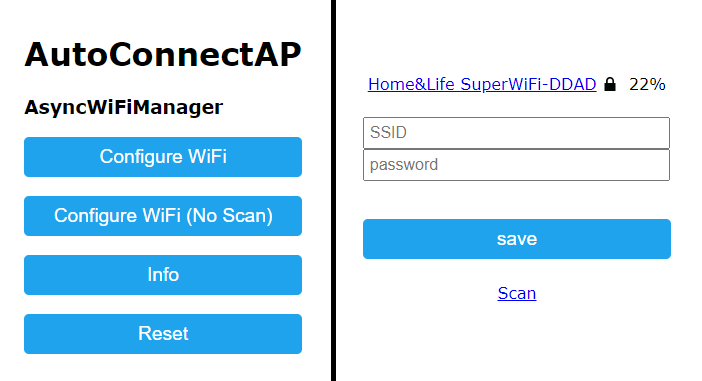
\includegraphics[width=\textwidth]{autoconnectap}
  \caption{Processo di inserimento credenziali WiFi tramite WiFiManager}
  \label{fig:autoconnectap}
\end{figure}

Successivamente viene tentata la connessione. Se non ha successo viene ripetuto lo stesso procedimento, altrimenti viene disattivato
l'Access Point temporaneo, avviene la connessione e il programma prosegue.

\subsection{Configurazione tramite form web}
Un'altra forma di modifica della configurazione è stata implementata tramite un web server configurato per mezzo della libreria
\texttt{ESPAsyncWebServer} ed esposto alla rete locale all'indirizzo IP o hostname del microcontrollore.
 Inizialmente la pagina conteneva un semplice form tramite il quale era possibile inviare un intero JSON
di configurazione, successivamente è stata aggiunta la possibilità di impostare i singoli parametri attraverso un form precompilato
e richieste AJAX. Un punto debole di questa soluzione è la scarsa flessibilità del web server, che gestisce richieste POST solo codificate
come Form Data, quindi invece che poter mandare un semplice JSON nel body della richiesta come da prassi con AJAX, è stato necessario
trasformarlo in FormData come valore associato alla chiave setFromJSON.
Nel dettaglio, erano esposti i seguenti endpoint:
\begin{itemize}
  \item /: Pagina di configurazione (index.html)
  \item /get/running-conf: Restituisce la configurazione attualmente in esecuzione in formato JSON
  \item /get/saved-conf: Restituisce il file di configurazione presente nella memoria flash
  \item /post: permette di inviare un intero JSON di configurazione (anche incompleto, vengono modificati solo i campi specificati) come
        valore associato alla chiave setFromJSON. È inoltre possibile associare alla chiave saveToFlash il valore `true' per copiare
        la configurazione in esecuzione nella memoria flash.
\end{itemize}
\noindent Si riporta in Figura~\ref{fig:confwebpage} la pagina di configurazione. 

\begin{figure}[h]
  \centering
  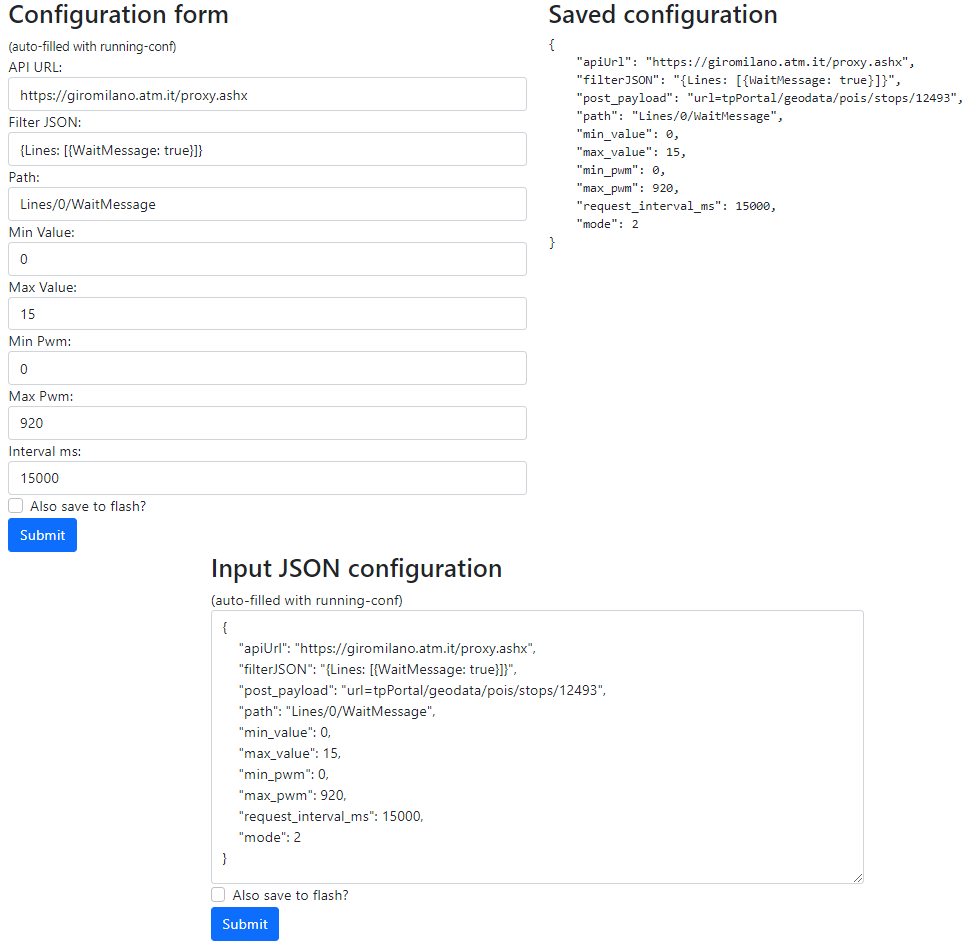
\includegraphics[width=\textwidth]{confwebpage}
  \caption{Pagina web di configurazione come si presentava quando abilitata}
  \label{fig:confwebpage}
\end{figure}

I form erano precompilati con la configurazione in esecuzione (\emph{running-conf}) ed era presente una sezione che riportava la
configurazione salvata nella flash (\emph{saved-conf}).
Le modifiche non erano automaticamente salvate nella memoria flash ma ciò doveva essere richiesto esplicitamente. Nei form di configurazione
era presente una checkbox da spuntare in caso si volesse che questo avvenisse.

Questa feature è successivamente stata disattivata perché l'esecuzione contemporanea di un webserver e di richieste API creava
problemi di allocazione della memoria del microcontrollore che spesso risultavano in crash improvvisi. Oltretutto, la spartana
interfaccia web risultava ridondante rispetto alle modalità di configurazione già presenti in quanto non garantiva una maggiore
semplicità di utilizzo per l'utente, che deve essere comunque esperto per apportare certe modifiche.

\subsection{Server FTP}
È stato aggiunto un rudimentale server FTP che consente di interagire con il file system del microcontrollore. Risulta molto utile per
l'upload, la rimozione e la modifica dei file JSON di configurazione e del file \texttt{confselect}, che contiene al suo interno il nome
del file di configurazione da utilizzare come attivo.

\subsection{OTA}
Sono stati implementati gli aggiornamenti OTA (Over the Air), processo tramite il quale è possibile eseguire l'upload di firmware
mediante WiFi invece che tramite porta seriale. Questo rimuove l'obbligo di utilizzo di una connessione cablata ed è molto utile
in situazioni di difficile accesso fisico al microcontrollore.

Il processo di upload usa Digest-MD5 per la verifica dell'integrità, onde evitare di rendere il dispositivo inservibile. È inoltre possibile
migliorare la sicurezza dell'operazione mediante utilizzo di password e hash firmati. \cite{espota}

\section{Implementazione modalità Smart Home}
%\todo{atrent: cambiare titolo e riempire, ESPHOME con spiegazione dello yaml}
Questa modalità era stata inizialmente pensata come complemento della modalità API: condivideva in parte i parametri di configurazione
e consisteva nel mappare in uscita sullo strumento, al posto di un valore ritornato dalle API, un valore passato tramite messaggio MQTT
a uno specifico topic (\texttt{<root>/setValue}).
Questo perché date le scarse risorse dell' ESP e l'impossibilità di generalizzare ogni forma di ottenimento dati in modalità standalone,
si è voluto offire la possibilità di effettuare ricerche ed elaborazioni fuori dal microcontrollore e passare un risultato ``già pronto"
come messaggio.

Andando avanti con le idee di sviluppo era in cantiere un'estensione del programma per l'integrazione nello scambio di messaggi di
componenti aggiuntive quali switch, commutatori, ecc. già descritte in altre sezioni.
Questo avrebbe voluto dire scrivere codice per ogni tipo di componente aggiuntivo da integrare nel sistema e trovare un modo per
abilitare solo il necessario in base alla configurazione fisica del dispositivo,
il tutto in ottica di una possibile integrazione con sistemi di domotica per il raccoglimento e l'elaborazione dei dati dei vari sensori e input.

Questa lista di funzionalità rispecchia molto bene quella di ESPHome, per cui è stato relegato il funzionamento standalone del solo ago
con codice scritto su misura alla ``modalità API", mentre per un'integrazione con sistemi di domotica e la gestione di vari input e output
sempre diversi si è scelto di fare totale affidamento su ESPHome, che grazie alla sua estensiva documentazione e compatibilità con una
vasta gamma di componenti esterne si presta molto bene all'incarico.

In particolare, la configurazione avviene per mezzo di file YAML in cui è possibile dichiarare proprietà e componenti utilizzati:

\begin{lstlisting}[language=yaml]
esphome:
  name: iotdial-aabbccdd
  platform: ESP8266
  board: d1_mini
  esp8266_restore_from_flash: yes

wifi:
  ssid: !secret wifi_ssid
  password: !secret wifi_password

  # Enable fallback hotspot (captive portal) in case wifi connection fails
  ap:
    ssid: "Iotdial Fallback Hotspot"
    password: "IoTDial!"
captive_portal:
\end{lstlisting}
Questa prima parte di configurazione specifica nome e piattaforma, dichiara inoltre una coppia ssid/password per la rete WiFi
e abilita l'access point di scorta, in maniera simile alla modalità API. Le credenziali della rete sono memorizzate in un file apposito
denominato secrets.yaml:
\begin{lstlisting}[language=yaml]
wifi_ssid: "IOT_TEST"
wifi_password: "IOT_TEST"
\end{lstlisting}

Nell'implementazione tramite ESPHome permangono le 4 variabili globali già viste nell'implementazione della modalità API:
min_value, max_value, min_pwm e max_pwm, per un mapping del valore da rappresentare sullo strumento.
La differenza sta in min_pwm e max_pwm che invece di seguire un intervallo tra 0 e 1023 sono rappresentate in ESPHome come una
percentuale, da 0.00 a 1.00. Segue la dichiarazione delle variabili globali:
\begin{lstlisting}[language=yaml]
globals:
  - id: min_value
    type: float
    restore_value: yes
    initial_value: '0'

  - id: max_value
    type: float
    restore_value: yes
    initial_value: '40'

  - id: min_pwm
    type: float
    restore_value: yes
    initial_value: '0'

  - id: max_pwm
    type: float
    restore_value: yes
    initial_value: '0.89'
\end{lstlisting}
La flag restore_value, accoppiata con esp8266_restore_from_flash presente all'inizio, serve per comunicare l'intenzione di mantenere
lo stato di queste variabili in maniera persistente ai riavvii, in modo che le modifiche non vadano perse.

Per la ricezione di valori e configurazioni tramite MQTT è stato configurato il broker:
\begin{lstlisting}[language=yaml]
mqtt:
  broker: mqtt.atrent.it
  topic_prefix: IoTDial/busolin
  discovery: True #homeassistant
\end{lstlisting}
La sottoscrizione a topic MQTT viene effettuata mediante dei componenti sensor ``virtuali":
\todo{busolin: usare map()}
\begin{lstlisting}[language=yaml]
sensor:
  - platform: mqtt_subscribe
    name: "Temperatura"
    id: temperatura
    topic: fuori_come_un_balcone/temp
    on_value:
      then:
        - output.set_level:
            id: dial
            level: !lambda "return map(x, id(min_value), id(max_value), id(min_pwm), id(max_pwm))/100.0;"

  - platform: mqtt_subscribe
    name: "setMinValue"
    id: setMinValue
    topic: IoTDial/busolin/settings/setMinValue
    on_value:
      then:
        - lambda: "id(min_value)=x;"
\end{lstlisting}
Nel dettaglio, in questo frammento viene effettuata una sottoscrizione ad un topic in cui viene periodicamente pubblicata
la rilevazione della temperatura esterna e utilizzando un piccolo script viene mappato il valore a un'uscita PWM sfruttando le variabili
globali.
Successivamente si può osservare una sottoscrizione creata per l'aggiornamento della variabile globale min_value (ne sono presenti
per tutte e quattro le variabili). In caso per qualche motivo l'intervallo dei valori cambi (ad esempio per un cambio di stagione) è
possibile eseguire questa modifica che grazie alle impostazioni precedentemente prescritte viene mantenuta in memoria flash.

L'output verso il voltmetro è dichiarato nel seguente modo:
\begin{lstlisting}[language=yaml]
output:
  - platform: esp8266_pwm
    pin: D2
    id: dial
\end{lstlisting}

Ai topic figli di topic_prefix verranno automaticamente pubblicati gli stati di ogni sensore fisico e virtuale configurati nello YAML,
quindi per un'integrazione con sistemi di domotica basta aggiungere un elemento sotto sensors e attivare la sottoscrizione al
topic che esso genererà.

Altri input e output aggiunti a ESPHome perché presenti sullo strumento a seguito delle modifiche sono il LED RGB interno,
il commutatore modificato, il pulsante, l'indicatore LED esterno e il buzzer:
\begin{lstlisting}[language=yaml]
#LED RGB
light:
  - platform: fastled_spi
    chipset: WS2801
    data_pin: D3
    clock_pin: D4
    num_leds: 1
    rgb_order: BRG
    name: "RGB LED"

#Commutatore
sensor:
  - platform: adc
    pin: A0
    name: "Switch"
    update_interval: 5s
    id: switchone

#Pulsante
binary_sensor:
  - platform: gpio
    pin:
      number: D7
      mode: INPUT_PULLUP
      inverted: True
    name: "Pulsante"

output:
  #Buzzer
  - platform: esp8266_pwm
    pin: D5
    id: rtttl_out

  #LED Esterno
  - platform: gpio
    pin: D0
    id: led

rtttl:
  output: rtttl_out
\end{lstlisting}

ESPHome si integra anche nativamente con Home Assistant: uno dei sistemi di gestione della domotica più diffusi. In
Figura~\ref{fig:ha-iotdial} è possibile vedere come IoTDial viene riprodotto nel pannello di controllo. \todo{busolin: va bene qui?}

\begin{figure}[h]
  \centering
  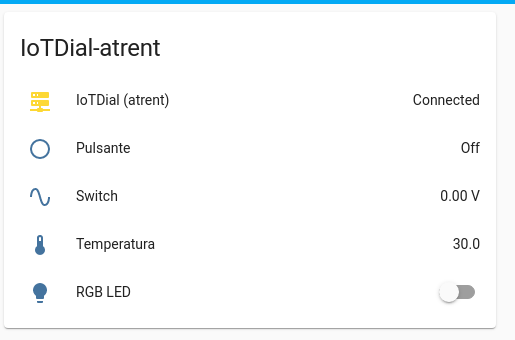
\includegraphics[width=0.8\textwidth]{ha-iotdial}
  \caption{IoTDial per come si mostra nel pannello di controllo di Home Assistant}
  \label{fig:ha-iotdial}
\end{figure}

\chapter{Conclusioni}
%\todo{atrent: oltre alla presentazione all'hacklab (domani!) proviamo a organizzare una sessione ad hoc almeno con gli studenti del corso SistEmbed (e magari quelli di PROS?)}

\section{Scelta dei dati da ``fisicalizzare"}
Durante la scelta dei dati che potrebbero essere oggetto di fisicalizzazione, mediante richieste API o integrazione con sistemi MQTT
del caso, è risultato evidente che bisogna pensare ai dati in maniera qualitativa, ossia considerando le limitate possibilità di visualizzazione
offerte dallo spostamento di un ago su una scala lineare bisogna ragionare su cosa sia significativo e comprensibile da visualizzare.

\section{Impressioni su IoTDial} %\todo{atrent: da qualche parte mettere i risultati dei questionari}
Per ottenere delle impressioni esterne sul lavoro svolto e raccogliere qualche idea di dati da fisicalizzare, sono state tenute un paio di
presentazioni prima con alcuni membri dell'HackLab Cormano e poi con alcuni studenti dei corsi di Sistemi Embedded della laurea triennale
in Informatica e Progettazione di Sistemi Operativi della magistrale.
Ai partecipanti è stato successivamente sottoposto un questionario in cui venivano proposte alcune idee di dati da fisicalizzare e per ciascuno
era chiesto un parare di adeguatezza di IoTDial in un intervallo da 1 a 5 considerando la scala da ``Per nulla adatto" a ``Molto adatto".
Successivamente erano esposti in ordine crescente di complessità/specificità i principi di funzionamento del prototipo e veniva chiesto per
ciascuno un intervallo da 1 a 5 di comprensione in una scala da ``Poco" a ``Molto".
Nella sezione finale veniva chiesto sempre in un intervallo da 1 a 5 quanto si potesse ritenere utile avere in casa un oggetto simile a quello
presentato e un paio di domande aperte relative a suggerimenti sui dati da rappresentare e altri suggerimenti più generali.

Il numero di risposte non è stato altissimo,  poco più di una decina.
Sicuramente ha influito molto il periodo di presentazione (giugno) in cui gran parte degli studenti hanno esami per cui prepararsi.
Hanno risposto per il 90\% uomini rientranti nelle fasce d'età 22-29 e 50-66. Nella prima fascia sono presenti solo studenti mentre nella
successiva impiegati e un pensionato.
Il livello generale di conoscenza dell'informatica è abbastanza alto mentre quello dell'elettronica è medio-basso.

\noindent Le idee di visualizzazione su cui venivano chieste delle opinioni sono:
\begin{itemize}
  \item ``Remotizzare" una misurazione allontanandosi dalla posizione fisica del sensore
  \item Visualizzazione tempo rimanente all'arrivo del bus/tram/treno
  \item Visualizzare la probabilità di pioggia
  \item Visualizzare il traffico passante nella rete locale
  \item Visualizzare il consumo di corrente in appartamento
  \item Visualizzare la concentrazione di traffico sul percorso casa-lavoro (tanto per regolarsi su quando partire, ad esempio dando un'occhiata mentre ci si prepara)
\end{itemize}
Per tutte tranne l'ultima c'è stata una buona risposta generale, specialmente per quanto riguarda il consumo di corrente, mentre per l'ultima
c'è stata più incertezza e le risposte sono state più distribuite nell'intervallo. I risultati di questa sezione sono consultabili in
Figura~\ref{fig:adeguatezzavis}.
\begin{figure}[h]
  \centering
  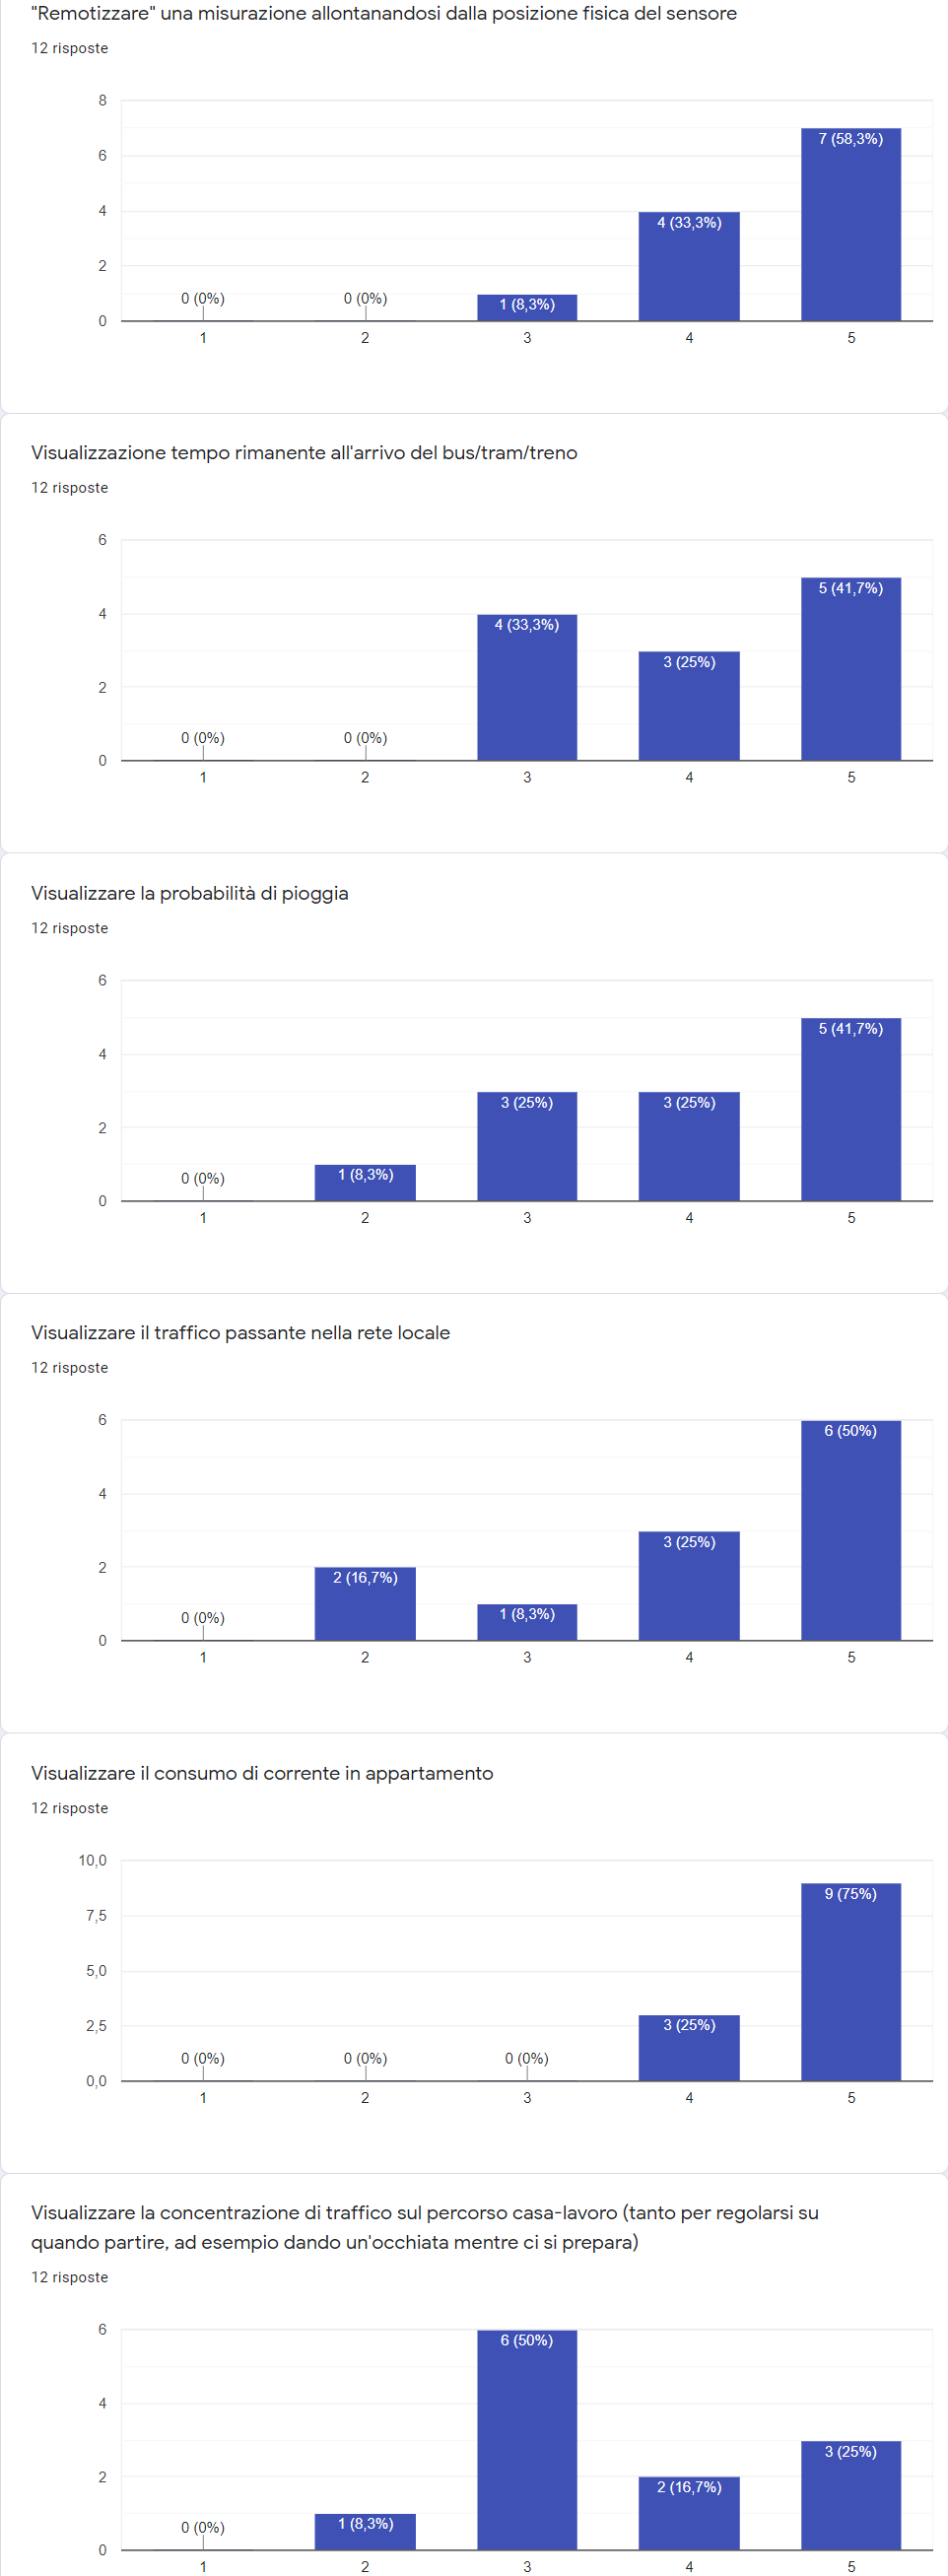
\includegraphics[width=\textwidth,height=0.95\textheight,keepaspectratio]{ressez2}
  \caption{Risultati della sezione sull'adeguatezza alla visualizzazione di certi dati}
  \label{fig:adeguatezzavis}
\end{figure}

I principi di funzionamento sono quasi tutti stati afferrati almeno a livello medio dalla quasi totalità dei partecipanti. Nel dettaglio la lista è:
\begin{itemize}
  \item Utilizzare uno strumento ad ago come visualizzatore di dati
  \item Utilizzare un microcontrollore per pilotare lo strumento mediante una differenza di potenziale variabile
  \item Effettuare richieste ad API su Internet da un dispositivo embedded
  \item Modificare le impostazioni di ottenimento dei dati mediante meccanismi di messaggistica quale MQTT
\end{itemize}
C'è stata un po' di titubanza sull'utilizzo di messaggistica MQTT per l'alterazione della configurazione.
I risultati di questa sezione sono consultabili in Figura~\ref{fig:comprensibilita}.
\begin{figure}[h]
  \centering
  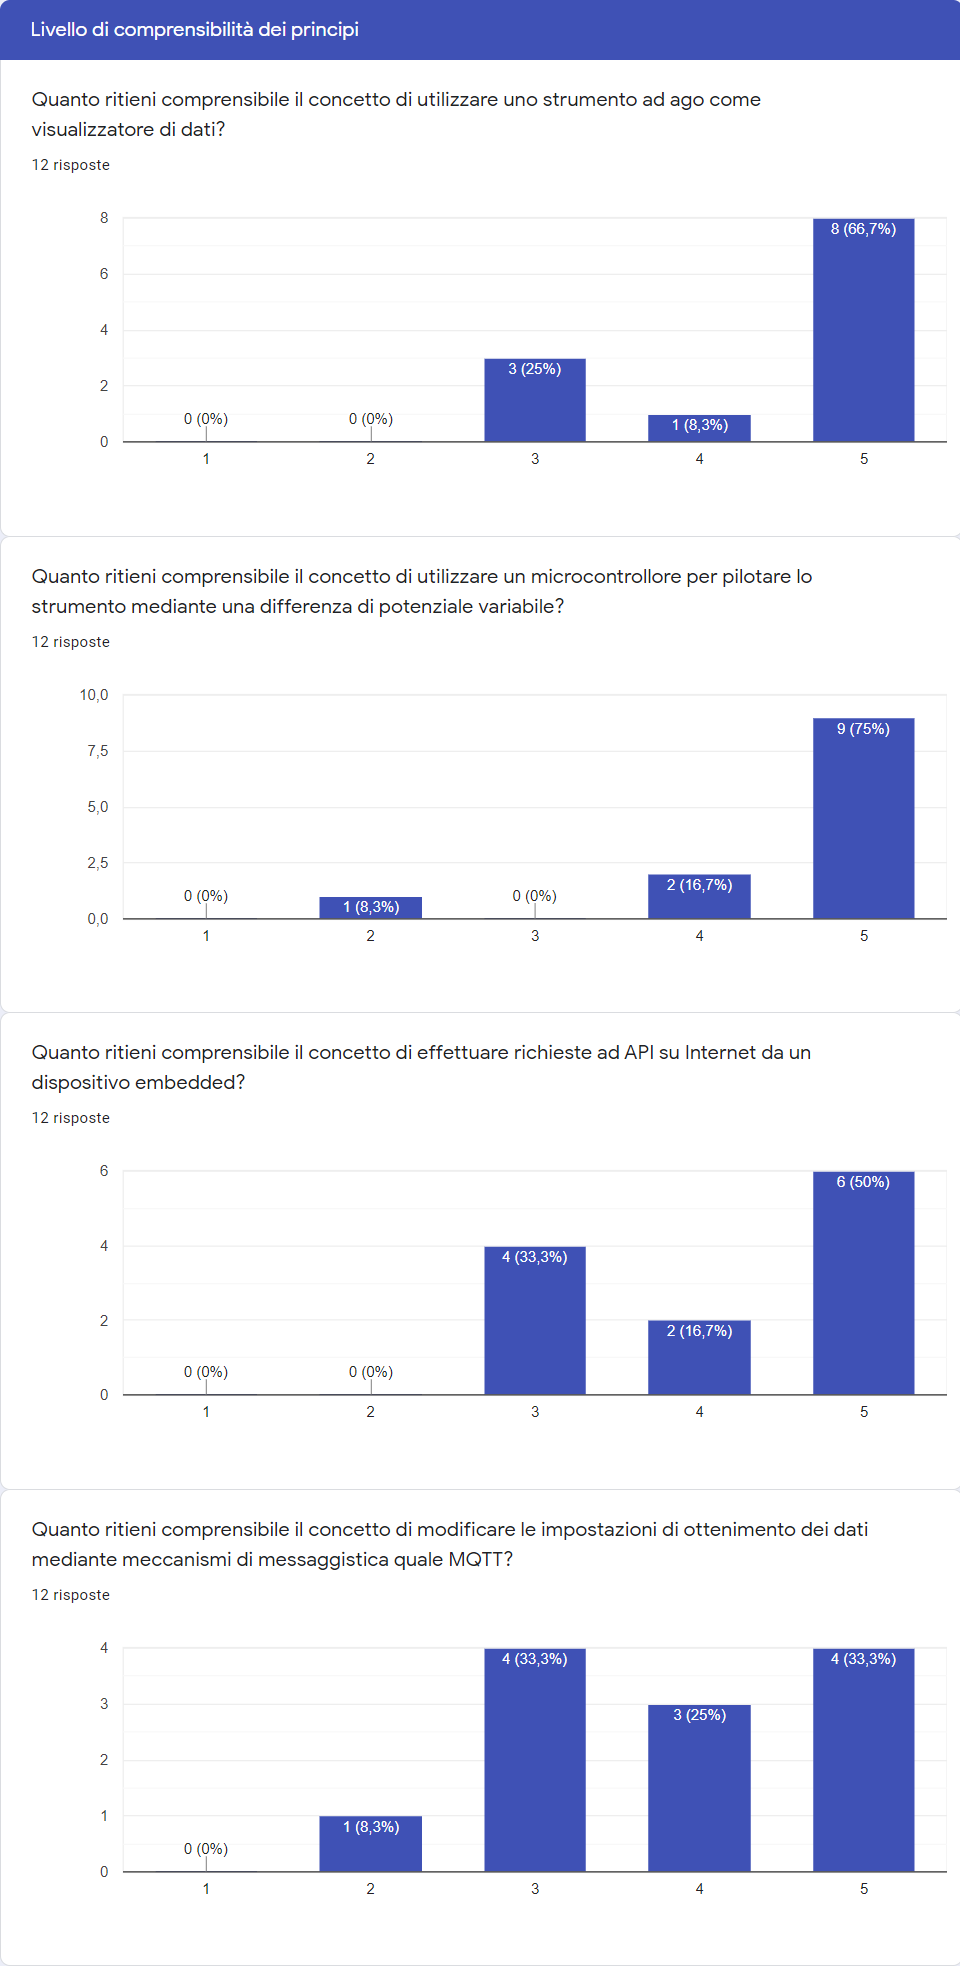
\includegraphics[width=\textwidth,height=0.95\textheight,keepaspectratio]{ressez3}
  \caption{Risultati della sezione sulla comprensibilità dei principi}
  \label{fig:comprensibilita}
\end{figure}

La sezione finale conteneva la domanda ``Quanto riterresti utile avere in casa un dispositivo simile a quello presentato nella demo che
funga sia da soprammobile che da fonte di informazioni slegata dai classici device (PC/Smartphone)?", a cui sono arrivati pareri abbastanza
uniformi nella scala 2-5. Suggerimenti aggiuntivi su dati che potrebbero essere oggetto di visualizzazione hanno restituito:
\begin{itemize}
  \item Utilizzo di CPU/RAM/GPU, altre statistiche ottenibili con lm_sensors e strumenti simili
  \item Alba$\div$tramonto
  \item Temperatura frigo o forno
  \item Qualsiasi altro sensore legato al meteo (es: vento)
  \item Tempo all'arrivo di un taxi o di un autista
  \item Ping dalla rete locale ad un server esterno
  \item Numero di email non lette nella propria casella via pop/imap (o messaggi su vari servizi, es telegram)
  \item Valore di una (cripto)valuta, un titolo azionario o simili tramite API di servizi appositi
  \item Affollamento attuale di un luogo (ristorante, bar, ufficio postale, ecc) tramite scraping di "orari di punta" di Google
  \item Giorni rimanenti ad una scadenza (es. esame, consegna progetto, ecc)
\end{itemize}
Non sono stati inseriti suggerimenti generali nella sezione ``altri suggerimenti".

\section{Reperibilità delle API}
Durante la ricerca di API rappresentabili mediante Data Physicalization è risultato evidente che molte di quelle più congeniali non
sono pubbliche e spesso sono anche di difficile utilizzo. L'esperienza personale è stata con quelle di ATM per ottenere i minuti rimanenti
all'arrivo di un mezzo pubblico ma altri si sono scontrati con quelle di Trenitalia \cite{trenitaliashock}.

\subsection{Dettagli su ATM}

%\todo{atrent: metti qualche screenshot almeno...}
Le API di ATM sono usate per \href{https://giromilano.atm.it}{Giromilano} e l'unico modo per comprenderne il funzionamento è utilizzare
gli strumenti del browser per leggere le richieste e le risposte che vengono scambiate tra client e server durante la ricerca di un
percorso o di informazioni su una fermata specifica - Figura~\ref{fig:giromilanoconsolel}.

\begin{figure}[h]
  \centering
  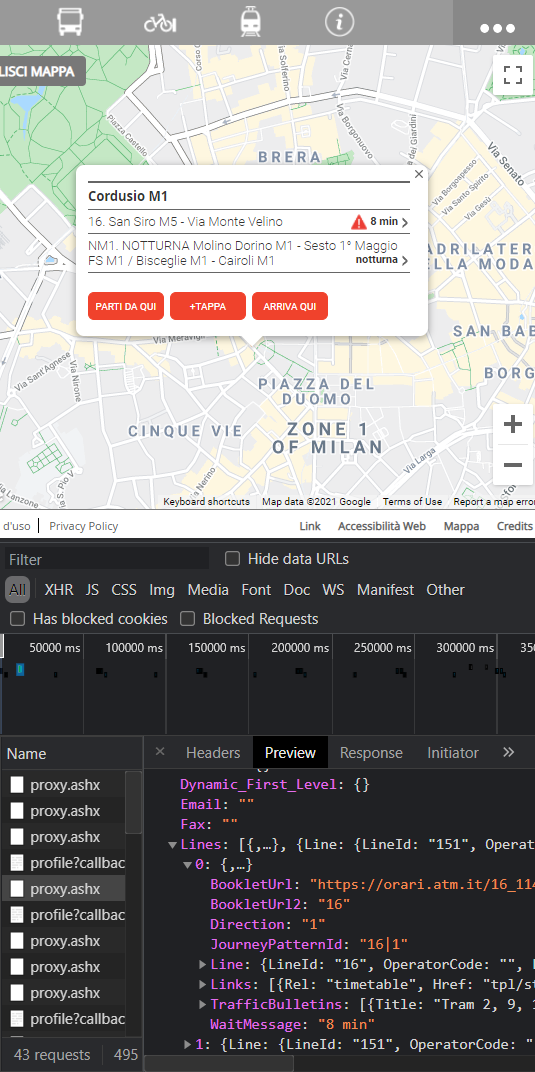
\includegraphics[width=\textwidth]{giromilanoconsole}
  \caption{Screenshot del sito di Giromilano con aperta la console sviluppatore del browser al fine di analizzare le richieste}
  \label{fig:giromilanoconsolel}
\end{figure}


In particolare per ottenere i minuti rimanenti all'arrivo di un mezzo ad una specifica fermata, è necessario effettuare una richiesta
POST a\\ \url{https://giromilano.atm.it/proxy.ashx} e nel body inserire\\ \texttt{url=tpPortal/geodata/pois/stops/xxxxx}, dove a
\texttt{xxxxx} va sostituito il numero della fermata, leggibile (a volte) nel mondo reale sulla pensilina o sul cartello o direttamente
dal sito.\\
Per ottenere una risposta è inoltre necessario inviare l'header\\ \texttt{Content-Type: application/x-www-form-urlencoded}
(proprio a questo fine è stata aggiunta la ``Modalità Fantozzi", che differisce dalla modalità API solamente per l'invio aggiuntivo
di questo header).
A questo punto sorgono alcuni problemi:
\begin{itemize}
  \item Le risposte contengono un po' di tutto e per via degli avvisi comprensivi di tag HTML possono anche essere molto lunghe, anche
        decine di kb - Figura~\ref{fig:giromilano-correctreq}.
  \item In caso di richiesta non corretta, ad esempio mancante di header Content-Type, non si avranno in risposta codici HTTP specifici
        ma sempre 200 (OK) in cui però la risposta è vuota - Figura~\ref{fig:giromilano-missingheader}.
\end{itemize}

\begin{figure}[h]
  \centering
  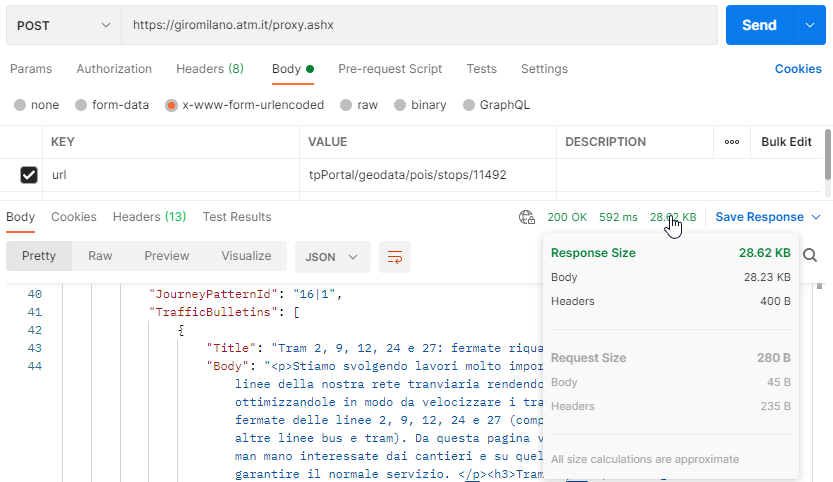
\includegraphics[width=\textwidth]{giromilano-correctreq}
  \caption{Richiesta ben impostata a Giromilano per la fermata 11492 - Cordusio M1. Notare la dimensione di 28KB della risposta}
  \label{fig:giromilano-correctreq}
\end{figure}

\begin{figure}[h]
  \centering
  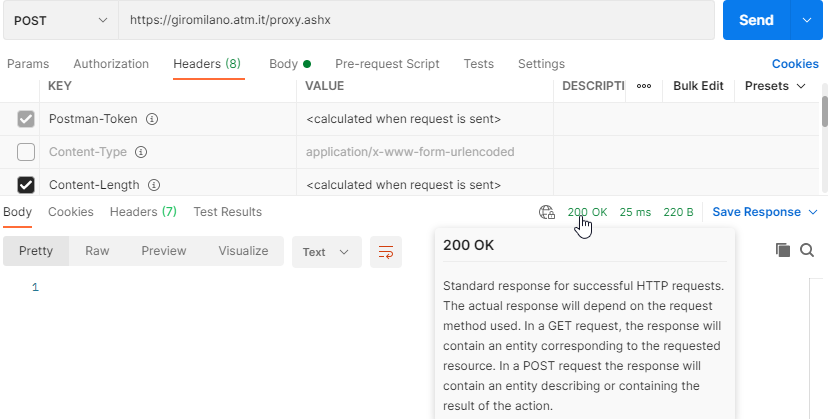
\includegraphics[width=\textwidth]{giromilano-missingheader}
  \caption{Richiesta simile a quella in Figura~\ref{fig:giromilano-correctreq} a meno dell'header mancante. Notare la risposta vuota ma il codice d'errore 200 - OK}
  \label{fig:giromilano-missingheader}
\end{figure}


A prescindere dalle questioni tecniche il problema è anche legale: non essendo API pubbliche l'utilizzo che se ne può fare all'esterno
dell'ambito aziendale è molto limitato. Può andare bene per utilizzi sperimentali personali, ma non si possono certamente incorporare
in prodotti da distribuire a qualsiasi titolo.
Poter risalire al ritardo accumulato da un mezzo pubblico (specialmente per treni con cadenza oraria o semioraria) senza dover navigare
siti e app ma direttamente lanciando un'occhiata a un angolo della stanza, come si farebbe con un orologio, sarebbe una comodità in più
per i pendolari che al momento non è attuabile su larga scala da terzi e le aziende di trasporti non sembrano interessate a proporre
prodotti simili.

\section{Sviluppi futuri}
Il prototipo realizzato durante il tirocinio, IoTDial, è solo un esempio di ciò che si può realizzare sulla base dell'idea di conversione degli
strumenti vintage, alcuni esempi di approcci diversi sono stati riportati nell'introduzione.

Un'idea di espansione di ciò che è stato fatto fino ad ora sarebbe utilizzare strumenti più grossi e con più input/indicatori per creare
una sorta di pannello di controllo domestico integrato con la domotica, che grazie a ESPHome sarebbe abbastanza immediato.
Ulteriori trasformazioni e utilizzi sono limitati solamente dalla fantasia.


\bibliographystyle{plain}
\bibliography{Biblio}
\addcontentsline{toc}{chapter}{Bibliografia}

\end{document}
